\documentclass[11pt,a4paper]{article}
\usepackage[utf8]{inputenc}
\usepackage[margin=0.85in]{geometry}
\usepackage{amsmath,amssymb}
\usepackage{graphicx}
\usepackage{booktabs}
\usepackage{microtype}
\usepackage{caption}
\usepackage{float}
\usepackage{hyperref}
\usepackage{xurl}
\usepackage{xcolor}
\usepackage{tabularx}
\usepackage{enumitem}
\usepackage{tocloft}
\usepackage{chngcntr}

\numberwithin{table}{section}
\numberwithin{figure}{section}

\setlength{\cftbeforesecskip}{3.5pt}
\setlength{\cftbeforesubsecskip}{1pt}

\hypersetup{
    colorlinks=true,
    linkcolor=blue!75!black,
    citecolor=blue!75!black,
    urlcolor=blue!75!black
}

\setlength{\parskip}{0.45em}
\setlength{\parindent}{0pt}

\title{\textbf{\LARGE ML-Driven PVT-Variation-Aware Leakage Estimation:\\Project Report}\\[0.5em]
\large Hierarchical Bottom-Up Modeling in 16nm LP CMOS for an 8-Bit Parity Checker}

\author{
\textbf{Course:} Digital VLSI Design --- Course Project\\[0.2em]
\textbf{Student / Author:} [FILL IN: Student Name / ID]\\[0.2em]
\textbf{Instructor / Faculty:} [FILL IN: Instructor Name / Faculty]\\[0.2em]
\textbf{Team / Group:} [FILL IN: Team Name / ID]\\[0.2em]
\textbf{Technology:} 16nm Low-Power (LP) CMOS (PTM BSIM4 Level 54, Nominal $V_{DD} = 1.0\,\mathrm{V}$)\\[0.2em]
\textbf{Target Circuit:} 8-Bit Parity Checker (28 NAND2 Gates, 112 Transistors)
}
\date{November 2026}

\begin{document}

\maketitle

\begin{abstract}
We built a hierarchical bottom-up machine-learning framework that predicts the static leakage current of CMOS circuits under process, voltage, and temperature (PVT) variations, and verified it against transistor-level SPICE simulations on a 16nm Low-Power (LP) technology at a nominal 1.0V supply ($V_{DD} \in [0.90, 1.10\,\mathrm{V}]$, $T \in [-40^\circ\mathrm{C}, 125^\circ\mathrm{C}]$). The target benchmark circuit is an 8-bit parity checker tree composed of 28 NAND2 gates (112 transistors). In Tier 1, four per-terminal multi-layer perceptron (MLP) neural networks (NMOS ON, NMOS OFF, PMOS ON, PMOS OFF) were developed using 64$\times$64 $\tanh$ architectures with Adam optimization and second-order L-BFGS polish, incorporating rail-augmented training datasets. Terminal currents spanning 13 decades were learned in symmetric logarithmic target space ($T(I) = \operatorname{sign}(I)\log_{10}(1 + |I|/10^{-15})$), achieving coefficients of determination $R^2 \in [0.9983, 0.9998]$ on held-out test data. In Tier 2, the transistor models were composed hierarchically without retraining to estimate the static leakage of five standard-cell logic gates (INV, NAND2, NOR2, AND2, OR2) across 18 input states and 200 random PVT corners (3,600 SPICE simulations), achieving a mean accuracy of \textbf{99.28\%} (median relative error \textbf{0.51\%}, 95th-percentile error \textbf{1.98\%}, maximum error 12.8\%). Evaluated using ML-solved internal node voltages, gate-level mean accuracy reached \textbf{99.25\%} (median relative error 0.53\%, 95th-percentile error 2.08\%). In Tier 3, the framework was scaled to the complete 8-bit parity checker across all 256 input vectors at the same 200 corners (51,200 SPICE simulations), reaching a fully-ML mean accuracy of \textbf{99.46\%} (median relative error \textbf{0.43\%}, 95th-percentile error \textbf{1.57\%}, maximum error 4.0\%), and \textbf{99.49\%} when evaluated with SPICE-solved node voltages (median error 0.40\%, 95th-percentile error 1.33\%). The project target set in the brief was ``up to 99\% mean accuracy''; this target was reached across both gate and full-circuit levels (superseding the v1 baseline of 96.72\% on gates and 97.28\% on circuit). Standalone gate SPICE summation reproduced full-circuit SPICE to 99.98\% (median error 0.013\%), providing an uncoupled physical benchmark (diagnostic only, not an ML result) that inter-gate electrical loading is negligible for the tested 8-bit parity checker and evaluated PVT corners in static CMOS DC steady state.
\end{abstract}

\newpage
\begingroup
\setlength{\parskip}{0pt}
\tableofcontents
\endgroup
\newpage

\section{Introduction}
Static leakage current is the current a transistor draws while in steady state, and in nanoscale technologies it constitutes a major fraction of total chip power dissipation. In sub-20\,nm regimes, supply voltages scale aggressively ($\sim 1.0\,\mathrm{V}$), physical gate oxides approach atomic dimensions ($t_{oxe} \approx 1.2\,\mathrm{nm}$), and threshold voltages leave minimal headroom below the supply. Consequently, transistors that are turned off still conduct non-negligible current through multiple physical leakage paths. For battery-powered mobile devices and low-activity IoT nodes that reside predominantly in standby mode, static leakage dictates battery lifetime, while in high-performance processors, leakage accelerates thermal dissipation.

Compounding this challenge, leakage current is extraordinarily sensitive to manufacturing tolerances and operating conditions. Small fluctuations in threshold voltage ($\pm 10\%$), temperature swings from $-40^\circ\mathrm{C}$ to $125^\circ\mathrm{C}$, or supply droops of $\pm 10\%$ alter leakage by multiple orders of magnitude. In controlled parameter sweeps on the assigned 16\,nm LP model, the OFF-state leakage of an NMOS device increased by a factor of approximately 186 between cold ($-40^\circ\mathrm{C}$) and hot ($125^\circ\mathrm{C}$), while PMOS OFF leakage grew by approximately 15.5. Designers therefore require complete statistical leakage distributions across process, voltage, and temperature (PVT) corners rather than a single nominal figure.

The standard industrial approach relies on SPICE-level circuit simulation (e.g., \texttt{ngspice} with BSIM4 models). While physically rigorous, SPICE iteratively solves non-linear nodal equations via Newton-Raphson techniques, creating an intractable computational bottleneck. Even for an 8-bit parity checker (112 transistors), evaluating all 256 input vectors across 200 corners requires 51,200 separate SPICE simulations. In our benchmark, this required over 83 CPU-minutes of computation. An automated machine-learning surrogate evaluates the same 51,200 operating points in less than a second.

This project investigates whether machine-learning surrogates trained strictly on lightweight, isolated single-transistor simulations can be combined bottom-up, without any circuit-level retraining, to accurately predict the leakage of complex multi-gate digital circuits under wide PVT variations.

\section{The Task and Deliverables}
The project brief (\textit{Digital VLSI Design: ML-Driven PVT-Variation-Aware Leakage Estimation}) requires each team to construct an automated, bottom-up leakage estimation pipeline using an assigned technology model card, nominal supply voltage, and test circuit. The assignment comprises three sequential tiers:
\begin{enumerate}[noitemsep]
    \item \textbf{Part A (Transistor Models):} For four distinct operating states (NMOS ON, NMOS OFF, PMOS ON, PMOS OFF), generate 10,000 random samples, execute SPICE simulations to extract all four terminal currents ($I_d, I_g, I_s, I_b$), and train regression models. Compare four candidate model families on a validation set, select the optimal model per case, and evaluate final accuracy on a held-out test set.
    \item \textbf{Part B (Gate-Level Validation):} Simulate five standard CMOS logic gates (INV, NAND2, NOR2, AND2, OR2) across all valid input states at 200 random PVT corners (18 gate-input cases $\times$ 200 corners = 3,600 SPICE runs). Evaluate gate leakage using the pre-trained Part~A transistor models without any retraining.
    \item \textbf{Part C (Test-Circuit Validation):} Synthesize the assigned circuit (an 8-bit parity checker built exclusively from standard gates) as a complete 112-transistor netlist. Simulate all 256 input vectors across the 200 PVT corners (51,200 SPICE simulations) and compare against hierarchical ML predictions.
\end{enumerate}

The specification targets up to \textbf{99\% mean accuracy} ($100\% \times [1 - \mathrm{MAPE}]$). The required deliverables are organized into ten components:
\begin{enumerate}[noitemsep]
    \item Four transistor datasets (10,000 rows each) conforming to exact column ordering.
    \item Example SPICE netlists for single transistors, standard gates, and the test circuit.
    \item Physical data checks: Kirchhoff's current law residuals (Figure~\ref{fig:kirchhoff}) and three-panel physical sensitivity trend sweeps (Figure~\ref{fig:trends}).
    \item Model comparison table: 4 model families $\times$ 4 cases on the validation partition.
    \item Chosen models: test-set metrics, predicted-vs-SPICE scatter plots, and saved model artifacts.
    \item Gate results table covering all 18 gate-input cases across 200 corners.
    \item Gate-level parity plot on logarithmic axes.
    \item Test-circuit results table and parity plot across 51,200 simulations.
    \item Reproducible code package that regenerates the pipeline with fixed random seeds.
    \item This comprehensive technical project report.
\end{enumerate}

\section{Background Concepts}
\subsection{Physical Origins of Leakage Current}
In sub-20\,nm bulk CMOS, three primary quantum and thermal transport mechanisms contribute to static leakage:
\begin{enumerate}[noitemsep]
    \item \textbf{Subthreshold Leakage ($I_{\mathrm{sub}}$):} Diffusion-dominated carrier transport between source and drain when the gate-to-source voltage $V_{gs}$ is below the threshold voltage $V_{th}$. It depends exponentially on temperature ($\propto \exp(-qV_{th}/mkT)$) and scales with Drain-Induced Barrier Lowering (DIBL), wherein elevated drain bias pulls down the channel potential barrier.
    \item \textbf{Gate-Oxide Direct Tunneling ($I_{\mathrm{gate}}$):} Quantum-mechanical tunneling of electrons and holes directly through the ultra-thin physical gate dielectric ($t_{oxe} \approx 1.2\,\mathrm{nm}$). Tunnelling depends exponentially on electric field intensity and barrier thickness, contributing to both ON and OFF states.
    \item \textbf{Junction and Substrate Leakage ($I_{\mathrm{body}}$):} Reverse-biased diode leakage and band-to-band tunneling (BTBT) across heavily doped source/drain-to-well p-n junctions.
\end{enumerate}
In this work, \texttt{ngspice} extracts all four terminal currents ($I_d, I_g, I_s, I_b$), ensuring that all physical leakage mechanisms modeled by BSIM4 are accounted for.

\subsection{PVT Variations and Process Parameters}
Process, Voltage, and Temperature (PVT) variations encapsulate real-world operational uncertainties:
\begin{itemize}[noitemsep]
    \item \textbf{Process ($P$):} Five fundamental BSIM4 physical parameters are perturbed uniformly by $\pm 10\%$ around their nominal values: zero-bias threshold voltage ($v_{th0}$), gate-oxide thickness ($t_{oxe}$), channel doping concentration ($N_{dep}$), low-field carrier mobility ($\mu_0$), and source/drain junction depth ($X_j$). NMOS and PMOS process draws are drawn independently.
    \item \textbf{Voltage ($V$):} Supply voltage varies uniformly by $\pm 10\%$ ($V_{DD} \in [0.90, 1.10\,\mathrm{V}]$).
    \item \textbf{Temperature ($T$):} Operating junction temperature spans $-40^\circ\mathrm{C}$ to $125^\circ\mathrm{C}$ ($233.15\,\mathrm{K}$ to $398.15\,\mathrm{K}$).
\end{itemize}

\subsection{Simulation Tools and BSIM4 Options}
Simulations were performed using \texttt{ngspice} (recorded as ngspice-42; 42 and 43 gave identical currents on the four single-transistor example netlists) using the Predictive Technology Model (PTM) 16\,nm Low-Power BSIM4 model card (Level 54). Every generated SPICE netlist includes the mandatory convergence options:
\begin{center}
\texttt{.options gmin=1e-18 abstol=1e-18 reltol=1e-6 vntol=1e-9}
\end{center}
These tightened numerical tolerances prevent sub-femtoampere currents from being corrupted by simulator truncation noise.

\subsection{Kirchhoff's Current Law as a Physical Invariant}
By charge conservation in static steady state, the algebraic sum of all currents entering a four-terminal transistor must equal zero:
\begin{equation}
\sum I = I_d + I_g + I_s + I_b = 0
\end{equation}
We adopt the standard convention where current entering a transistor terminal is defined as positive: $I_{\mathrm{terminal}} = -I(V_{\mathrm{source}})$. Evaluating KCL residuals validates netlist wiring, sign conventions, and simulator convergence before training.

\subsection{The Transistor Stack Effect}
When multiple transistors are connected in series (such as the pull-down NMOS stack in a NAND2 gate or the pull-up PMOS stack in a NOR2 gate), internal intermediate nodes settle at non-rail voltages governed by the mutual leakage equilibrium of the stacked devices. The resulting intermediate node voltage raises the source potential of the upper device, inducing negative gate-to-source bias ($V_{gs} < 0$) and body-effect threshold elevation ($V_{bs} < 0$), thereby exponentially reducing leakage (the stack effect). Modeling these internal floating nodes without full SPICE constitutes a major technical challenge.

\subsection{Machine Learning Terminology and Metrics}
\begin{itemize}[noitemsep]
    \item \textbf{Partitioning:} Datasets are split into 70\% training (7,000 rows), 15\% validation (1,500 rows), and 15\% test (1,500 rows) with fixed random seed 42.
    \item \textbf{Symmetric Logarithmic Target (symlog) and Inverse Transformation:} Because currents span 13 decades ($10^{-17}\,\mathrm{A}$ to $10^{-4}\,\mathrm{A}$), standard linear MSE regression fails completely. Targets are mapped using:
    \begin{equation}
    T(I) = \operatorname{sign}(I)\log_{10}\left(1 + \frac{|I|}{I_0}\right), \quad I_0 = 10^{-15}\,\mathrm{A}
    \end{equation}
    Model predictions in transformed space are mapped back to physical currents in amperes via the exact analytical inverse transformation:
    \begin{equation}
    I(T) = \operatorname{sign}(T) \cdot I_0 \cdot \left(10^{|T|} - 1\right)
    \end{equation}
    \item \textbf{Coefficient of Determination ($R^2$):} Measures variance explained. \textbf{Crucial distinction:} $R^2$ is evaluated strictly in the transformed symlog target space $T(I)$, evenly weighting sub-picoampere leakage and milliampere ON currents. Evaluating $R^2$ in raw amperes would make the metric sensitive only to large ON currents and blind to subthreshold leakage.
    \item \textbf{Relative Error and Mean Accuracy:} Evaluated on physical currents in amperes obtained from the inverse transformation with a $10^{-15}\,\mathrm{A}$ noise floor ($R^2$ is calculated in transformed symlog target space, while median and p95 relative errors are calculated on currents in amperes):
    \begin{equation}
    \text{RelErr} = \frac{|I_{\mathrm{pred}} - I_{\mathrm{true}}|}{\max(|I_{\mathrm{true}}|, 10^{-15}\,\mathrm{A})}, \quad \text{Mean Accuracy} = 100\% \times \left(1 - \frac{1}{N}\sum \text{RelErr}\right)
    \end{equation}
\end{itemize}

\section{Technology Setup and Operating Ranges}
Table~\ref{tab:tech_setup} details the nominal technology parameters, variation ranges, and simulation environment assigned to this project.

\begin{table}[H]
\centering
\caption{Assigned 16\,nm LP Technology and Simulation Parameters}
\label{tab:tech_setup}
\resizebox{\linewidth}{!}{
\begin{tabular}{lll}
\toprule
\textbf{Parameter} & \textbf{Symbol} & \textbf{Assigned Value / Range} \\
\midrule
Technology Model & -- & PTM 16nm\_LP.pm (BSIM4 Level 54, $T_{\mathrm{nom}} = 27^\circ\mathrm{C}$) \\
Nominal Supply & $V_{DD}$ & $1.0\,\mathrm{V} \pm 10\%$ ($0.90\,\mathrm{V} \text{ to } 1.10\,\mathrm{V}$) \\
Channel Length & $L_{\min}$ & $16\,\mathrm{nm}$ \\
Transistor Width & $W$ & $16\,\mathrm{nm} \text{ to } 128\,\mathrm{nm}$ ($1\times \text{ to } 8\times L_{\min}$, uniform sweep) \\
Operating Temperature & $T$ & $-40^\circ\mathrm{C} \text{ to } 125^\circ\mathrm{C}$ ($233.15\,\mathrm{K} \text{ to } 398.15\,\mathrm{K}$) \\
Target Benchmark Circuit & -- & 8-Bit Parity Checker (28 NAND2 Gates, 112 Transistors) \\
SPICE Simulation Engine & -- & \texttt{ngspice} (recorded as ngspice-42; 42 and 43 gave identical currents on the four single-transistor example netlists) \\
Software Stack & -- & Python 3.12, NumPy, SciPy, pandas, scikit-learn, joblib \\
\bottomrule
\end{tabular}
}
\end{table}

The nominal values and $\pm 10\%$ variation ranges of the five process parameters extracted directly from the \texttt{16nm\_LP.pm} model card are provided in Table~\ref{tab:proc_params}.

\begin{table}[H]
\centering
\caption{BSIM4 Process Parameters and Physical Variation Ranges ($\pm 10\%$ Uniform)}
\label{tab:proc_params}
\resizebox{\linewidth}{!}{
\begin{tabular}{lcccc}
\toprule
\textbf{Physical Parameter} & \textbf{NMOS Nominal} & \textbf{NMOS Range ($\pm 10\%$)} & \textbf{PMOS Nominal} & \textbf{PMOS Range ($\pm 10\%$)} \\
\midrule
Threshold Voltage ($v_{th0}$) & $+0.68191\,\mathrm{V}$ & $+0.61372 \text{ to } +0.75010\,\mathrm{V}$ & $-0.68620\,\mathrm{V}$ & $-0.75482 \text{ to } -0.61758\,\mathrm{V}$ \\
Oxide Thickness ($t_{oxe}$) & $1.20\,\mathrm{nm}$ & $1.080 \text{ to } 1.320\,\mathrm{nm}$ & $1.22\,\mathrm{nm}$ & $1.098 \text{ to } 1.342\,\mathrm{nm}$ \\
Channel Doping ($N_{dep}$) & $7.0\times 10^{18}\,\mathrm{cm}^{-3}$ & $6.30 \text{ to } 7.70\times 10^{18}$ & $4.4\times 10^{18}\,\mathrm{cm}^{-3}$ & $3.96 \text{ to } 4.84\times 10^{18}$ \\
Low-field Mobility ($\mu_0$) & $0.0280\,\mathrm{m}^2/\mathrm{V}\cdot\mathrm{s}$ & $0.0252 \text{ to } 0.0308$ & $0.0075\,\mathrm{m}^2/\mathrm{V}\cdot\mathrm{s}$ & $0.00675 \text{ to } 0.00825$ \\
Junction Depth ($X_j$) & $5.0\,\mathrm{nm}$ & $4.50 \text{ to } 5.50\,\mathrm{nm}$ & $7.2\,\mathrm{nm}$ & $6.48 \text{ to } 7.92\,\mathrm{nm}$ \\
\bottomrule
\end{tabular}
}
\end{table}

\section{Part A — Transistor Data Generation}
\subsection{The Four Transistor Operating States}
Transistors are sampled across four distinct terminal bias configurations as specified in Table~\ref{tab:trans_cases}.

\begin{table}[H]
\centering
\caption{The Four Transistor Operating States}
\label{tab:trans_cases}
\resizebox{\linewidth}{!}{
\begin{tabular}{lcccl}
\toprule
\textbf{Case Name} & \textbf{Gate Voltage ($V_g$)} & \textbf{Body Voltage ($V_b$)} & \textbf{Drain/Source ($V_d, V_s$)} & \textbf{Physical Circuit Role} \\
\midrule
NMOS ON  & $V_{DD}$ & $0\,\mathrm{V}$    & Uniform $[0, V_{DD}]$ & Conducting pull-down network transistor \\
NMOS OFF & $0\,\mathrm{V}$    & $0\,\mathrm{V}$    & Uniform $[0, V_{DD}]$ & Subthreshold blocking pull-down transistor \\
PMOS ON  & $0\,\mathrm{V}$    & $V_{DD}$ & Uniform $[0, V_{DD}]$ & Conducting pull-up network transistor \\
PMOS OFF & $V_{DD}$ & $V_{DD}$ & Uniform $[0, V_{DD}]$ & Subthreshold blocking pull-up transistor \\
\bottomrule
\end{tabular}
}
\end{table}

\subsection{Sampling Protocol and Dataset Validation}
Parameters are drawn sequentially using NumPy with fixed seed 42: $V_{DD} \sim \mathcal{U}(0.90, 1.10\,\mathrm{V})$ is drawn first, followed by temperature, width, and terminal voltages ($V_d, V_s \sim \mathcal{U}(0, V_{DD})$). The five process parameters are then drawn independently. To ensure 10,000 valid samples, 10,205 candidates were generated and simulated; exactly zero simulations failed. Automated duplicate scans confirmed zero duplicate input rows across all 40,000 samples.

\section{Checking the Data Before Trusting It}
\subsection{Kirchhoff's Current Law Validation (Table 6.1 and Figure 6.1)}
KCL residual checks were evaluated across all 40,000 transistor samples. Table~\ref{tab:kirchhoff} provides the exact residual metrics extracted from \path{results/PartA_transistor/kirchhoff_check.csv}.

\begin{table}[H]
\centering
\caption{Kirchhoff Current Law (KCL) Residual Validation Across 40,000 Samples}
\label{tab:kirchhoff}
\resizebox{\linewidth}{!}{
\begin{tabular}{lcccccc}
\toprule
\textbf{Case} & \textbf{Max Abs (A)} & \textbf{Median Abs (A)} & \textbf{Max Rel (\%)} & \textbf{Median Rel (\%)} & \textbf{p99 Rel (\%)} & \textbf{Fraction $< 10^{-3}\%$} \\
\midrule
NMOS ON  & $8.62\times 10^{-15}$ & $1.76\times 10^{-16}$ & 8.50\% & $1.39\times 10^{-8}\%$ & 1.41\% & 95.76\% \\
NMOS OFF & $5.65\times 10^{-21}$ & $3.72\times 10^{-25}$ & $1.02\times 10^{-8}\%$ & $1.53\times 10^{-9}\%$ & $8.36\times 10^{-9}\%$ & 100.0\% \\
PMOS ON  & $5.00\times 10^{-15}$ & $3.95\times 10^{-17}$ & 1.59\% & $7.98\times 10^{-9}\%$ & 0.34\% & 96.91\% \\
PMOS OFF & $2.28\times 10^{-15}$ & $1.53\times 10^{-16}$ & 26.02\% & $5.62\times 10^{-3}\%$ & 1.42\% & 89.27\% \\
\bottomrule
\end{tabular}
}
\end{table}

\textbf{Physical Analysis of KCL Residuals:} Absolute residuals stay below $8.62\times 10^{-15}\,\mathrm{A}$ across all four cases, confirming correct terminal wiring and sign conventions. In the PMOS OFF dataset, the maximum relative residual reaches 26.02\%, but this relative metric is artificially inflated because it occurs exclusively at operational points where all four terminal currents reside near the sub-femtoampere numerical noise floor ($|I| < 10^{-14}\,\mathrm{A}$). The corresponding maximum absolute residual across all 10,000 PMOS OFF simulations is only $2.28\times 10^{-15}\,\mathrm{A}$ (2.28\,fA), with a median absolute residual of $1.53\times 10^{-16}\,\mathrm{A}$ (0.153\,fA). Figure~\ref{fig:kirchhoff} shows the residual distributions.

\begin{figure}[H]
\centering
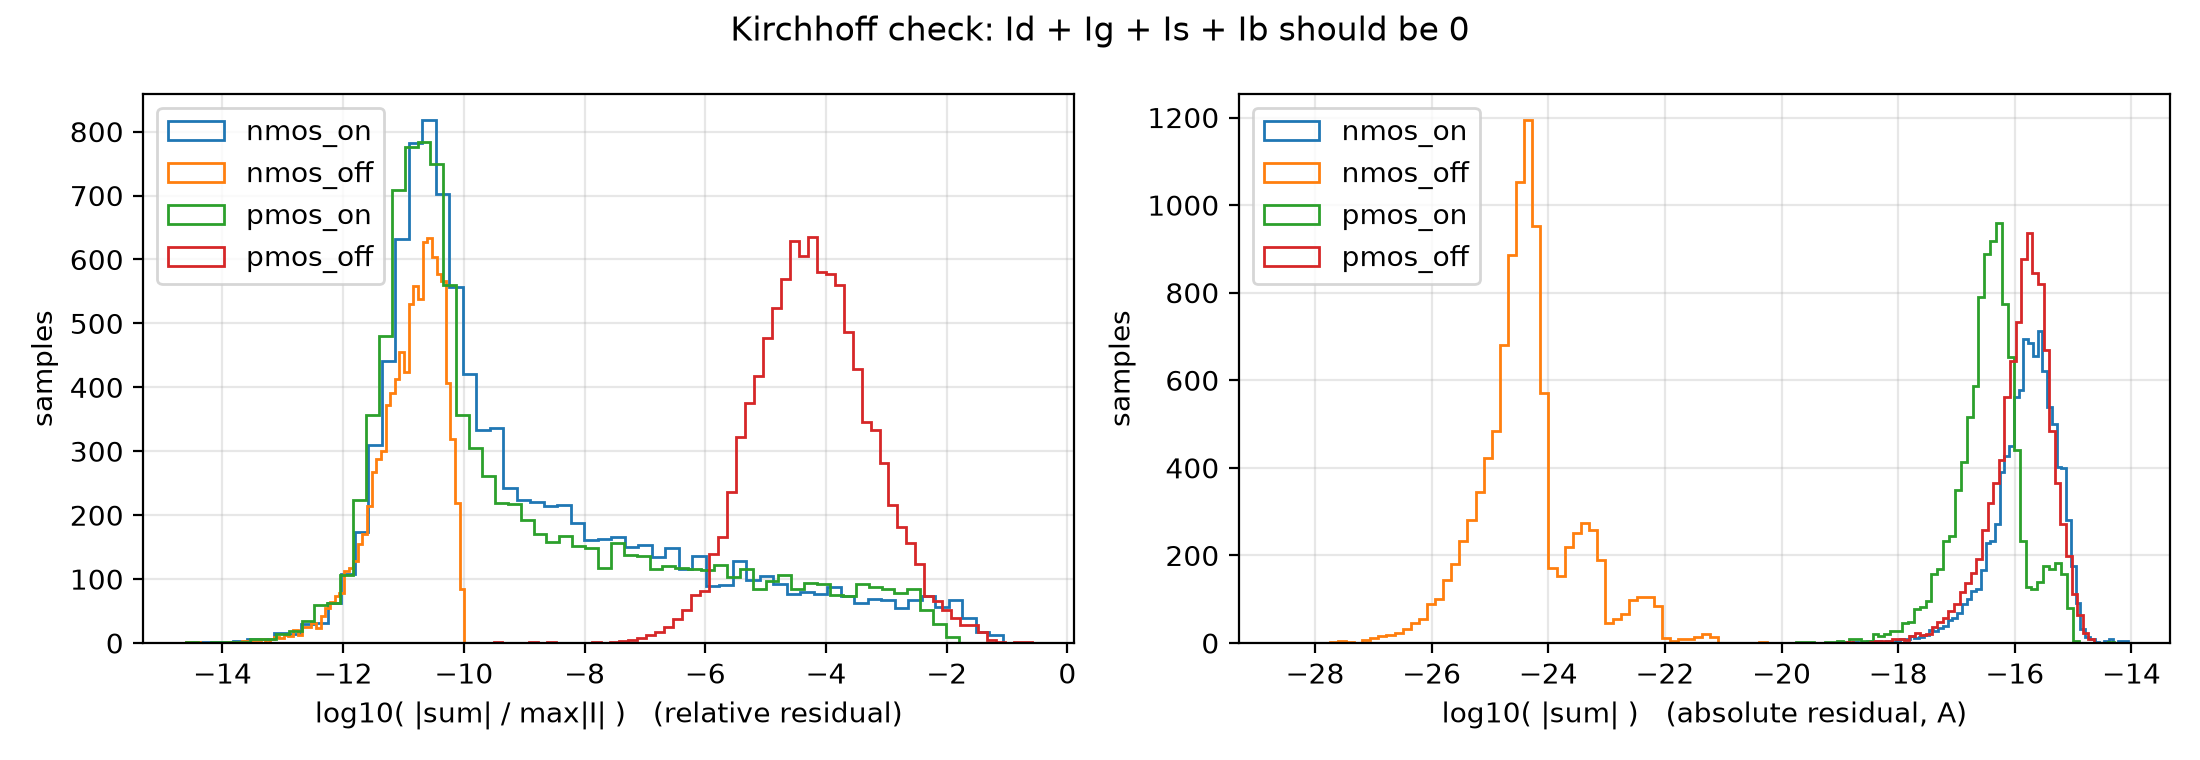
\includegraphics[width=0.85\textwidth]{../plots/PartA_transistor/kirchhoff_check.png}
\caption{Kirchhoff Current Law (KCL) absolute and relative residual distributions across the four transistor cases.}
\label{fig:kirchhoff}
\end{figure}

\subsection{Physical Trend Validation (Figure 6.2)}
To confirm device physics before training, three single-parameter controlled sensitivity sweeps were executed (\texttt{trends.py}) and compiled into the three-panel plot in Figure~\ref{fig:trends}:
\begin{enumerate}[noitemsep]
    \item \textbf{OFF Current vs. Temperature (Figure~\ref{fig:trends}, left panel):} Subthreshold leakage increases exponentially from $-40^\circ\mathrm{C}$ to $125^\circ\mathrm{C}$. In the sweep, NMOS OFF current rose by a factor of 186.3 and PMOS OFF current by 15.5.
    \item \textbf{OFF Current vs. $v_{th0}$ (Figure~\ref{fig:trends}, centre panel):} OFF leakage drops exponentially as threshold voltage magnitude increases by $\pm 10\%$.
    \item \textbf{Gate Current vs. $t_{oxe}$ (Figure~\ref{fig:trends}, right panel):} Direct tunneling current drops monotonically by over $3.5\times$ as oxide thickness increases by $\pm 10\%$.
\end{enumerate}

\begin{figure}[H]
\centering
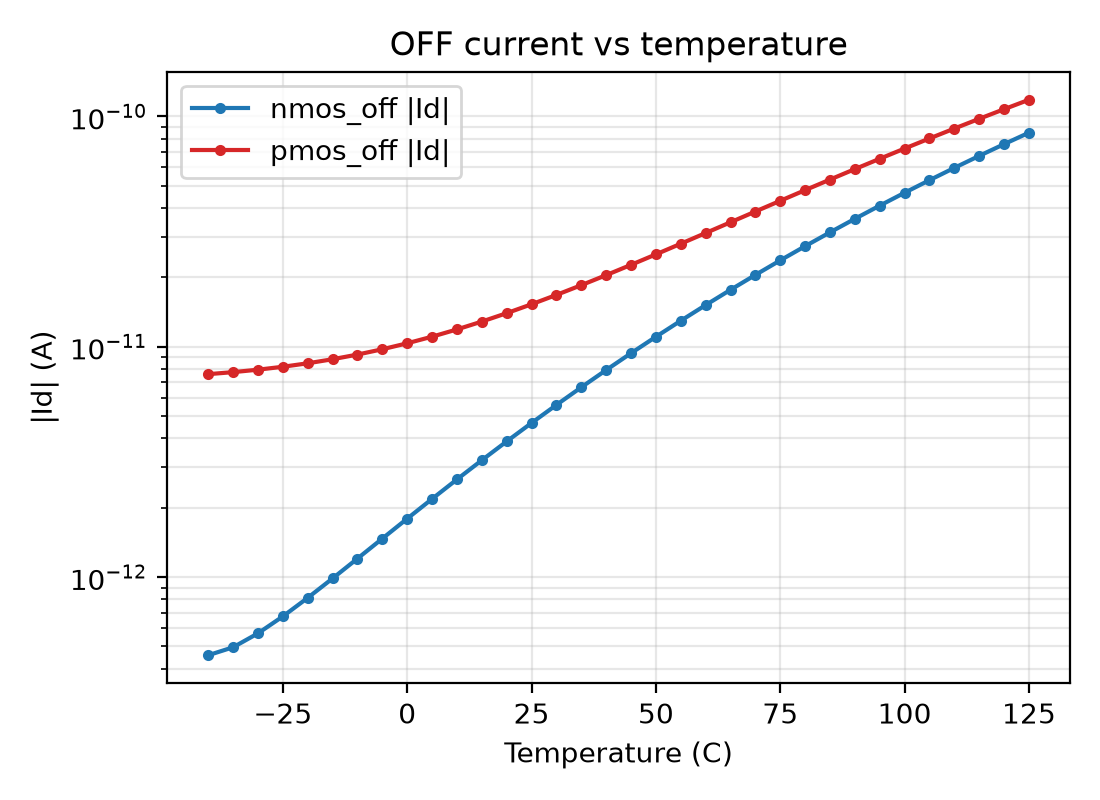
\includegraphics[width=0.32\linewidth]{../plots/PartA_transistor/trend1_off_current_vs_temperature.png}
\hfill
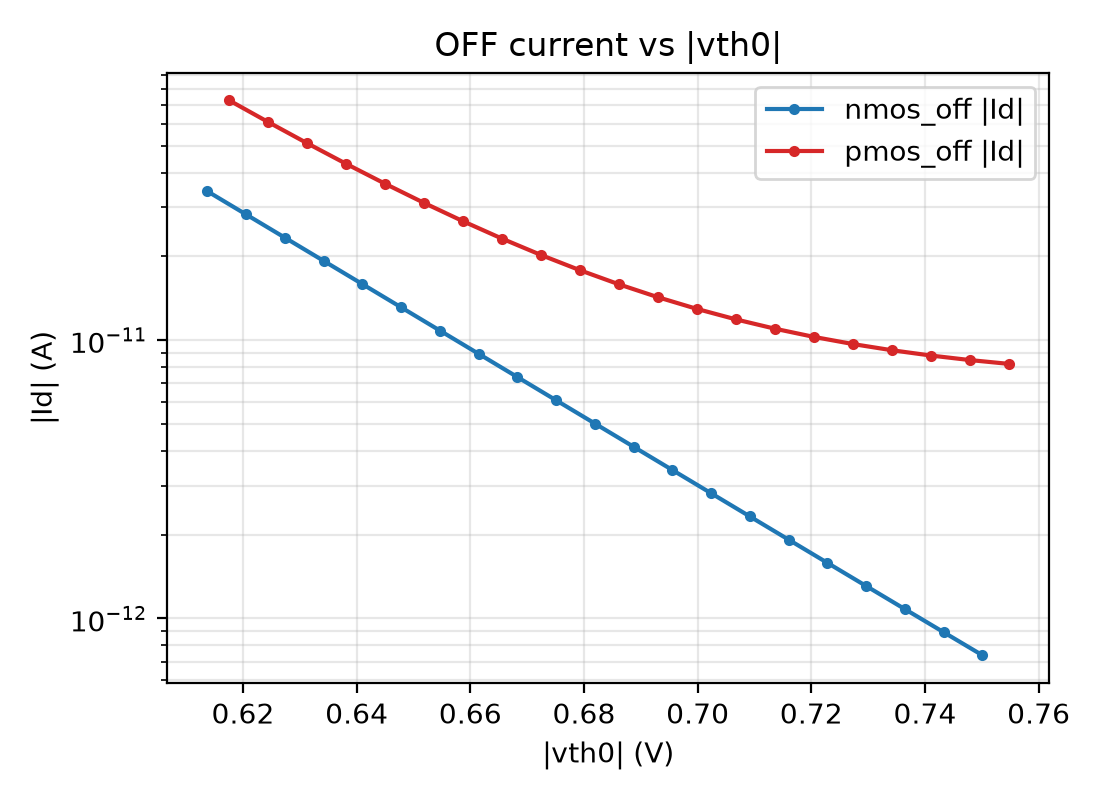
\includegraphics[width=0.32\linewidth]{../plots/PartA_transistor/trend2_off_current_vs_vth0.png}
\hfill
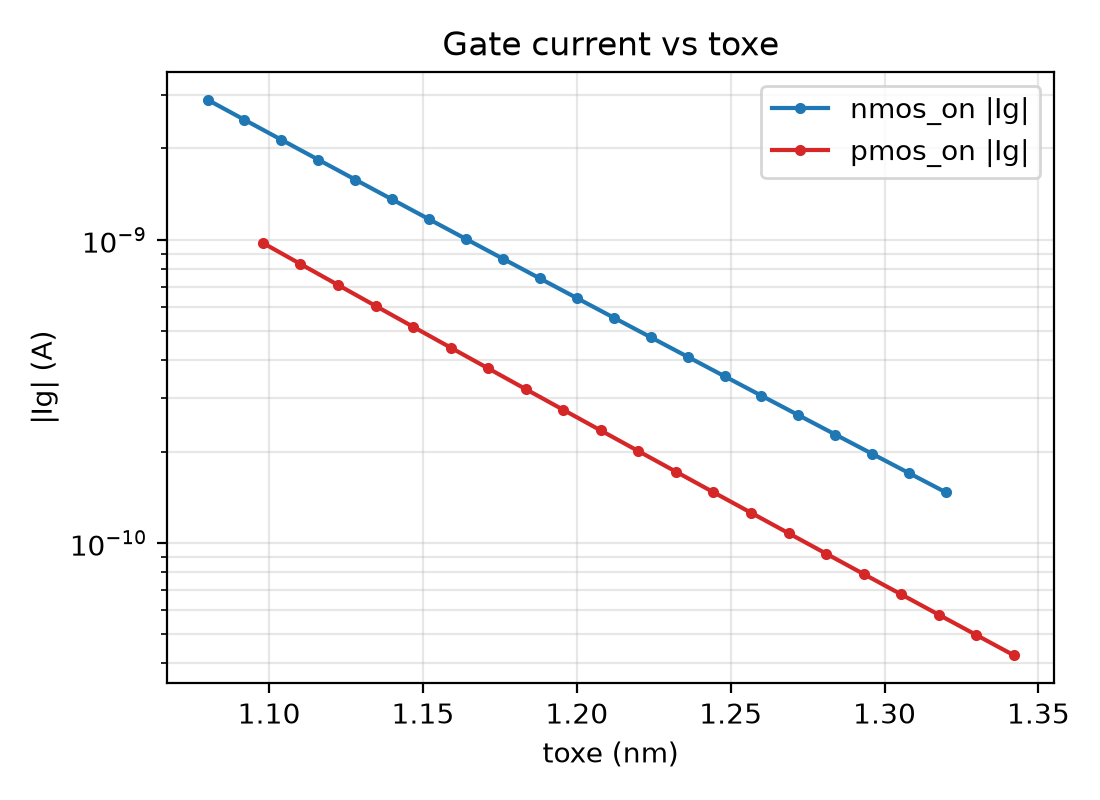
\includegraphics[width=0.32\linewidth]{../plots/PartA_transistor/trend3_gate_current_vs_toxe.png}
\caption{Physical trend validation sweeps: (left panel) subthreshold OFF leakage vs. temperature; (centre panel) subthreshold OFF leakage vs. $v_{th0}$; (right panel) gate direct tunneling leakage vs. oxide thickness $t_{oxe}$.}
\label{fig:trends}
\end{figure}

\section{Building the Transistor Models}
\subsection{Feature Engineering and Symmetric Logarithm}
The 12 raw inputs are expanded into 18 physically motivated features:
\begin{equation}
X_{\mathrm{feat}} = \left[\log_{10}(W), \frac{1000}{T + 273.15}, V_{ds}, V_{gs}, V_{gd}, V_{bs}, V_{bd}, V_{DD}, V_d, V_s, V_g, V_b, v_{th0}, t_{oxe}, N_{dep}, \mu_0, X_j\right]
\end{equation}
Targets are transformed into symmetric logarithmic target space $T(I)$ with $I_0 = 10^{-15}\,\mathrm{A}$.

\subsection{Model Comparison on Validation Set (Table 7.1)}
Four candidate model families were trained on 7,000 samples and compared on the 1,500 validation samples. Table~\ref{tab:model_comp} reproduces the complete 4 $\times$ 4 comparison from \path{results/PartA_transistor/model_comparison_validation.csv}.

\begin{table}[H]
\centering
\caption{Baseline (v1, Superseded) Validation Set Model Comparison Across 4 Cases (16 Models Evaluated)}
\label{tab:model_comp}
\resizebox{\linewidth}{!}{
\begin{tabular}{llccccc}
\toprule
\textbf{Case} & \textbf{Algorithm} & $\mathbf{R^2 (symlog)}$ & \textbf{Median Err. (\%)} & \textbf{p95 Err. (\%)} & \textbf{Training Time (s)} & \textbf{Selection Status} \\
\midrule
NMOS OFF & Poly Ridge (deg 3) & 0.9116 & 14.33\% & 185.16\% & 0.56 & Rejected \\
         & Random Forest (300) & 0.8551 & 0.24\% & 82.38\% & 26.53 & Rejected \\
         & Gradient Boosting & 0.9735 & 1.24\% & 67.41\% & 10.92 & Rejected \\
         & \textbf{MLP (128-128-64)} & \textbf{0.9977} & \textbf{0.56\%} & \textbf{12.24\%} & 157.28 & \textbf{Selected (Lowest p95)} \\
\midrule
NMOS ON  & Poly Ridge (deg 3) & 0.9122 & 84.57\% & 9176.11\% & 0.57 & Rejected \\
         & Random Forest (300) & 0.9806 & 29.45\% & 165.73\% & 15.84 & Rejected \\
         & Gradient Boosting & 0.9957 & 12.71\% & 66.21\% & 9.67 & Rejected \\
         & \textbf{MLP (128-128-64)} & \textbf{0.9982} & \textbf{4.87\%} & \textbf{28.46\%} & 180.55 & \textbf{Selected (Lowest p95)} \\
\midrule
PMOS OFF & Poly Ridge (deg 3) & 0.9367 & 15.53\% & 124.77\% & 0.56 & Rejected \\
         & Random Forest (300) & 0.9542 & 16.41\% & 86.43\% & 18.56 & Rejected \\
         & Gradient Boosting & 0.9828 & 4.37\% & 46.07\% & 9.27 & Rejected \\
         & \textbf{MLP (128-128-64)} & \textbf{0.9898} & \textbf{1.76\%} & \textbf{16.09\%} & 181.58 & \textbf{Selected (Lowest p95)} \\
\midrule
PMOS ON  & Poly Ridge (deg 3) & 0.9270 & 60.39\% & 10899.97\% & 0.61 & Rejected \\
         & Random Forest (300) & 0.9771 & 30.66\% & 189.06\% & 16.03 & Rejected \\
         & Gradient Boosting & 0.9962 & 13.09\% & 80.93\% & 9.66 & Rejected \\
         & \textbf{MLP (128-128-64)} & \textbf{0.9983} & \textbf{5.00\%} & \textbf{33.55\%} & 181.52 & \textbf{Selected (Lowest p95)} \\
\bottomrule
\end{tabular}
}
\end{table}

The Multi-Layer Perceptron (MLP) architecture (three hidden layers of 128, 128, and 64 neurons, ReLU activations, L-BFGS optimizer) won decisively in all four cases by minimizing the 95th-percentile error. Table~\ref{tab:new_vs_old_val} compares the baseline (v1) models against the verified upgrade (v2) on the exact 1,500 validation rows from \path{results/PartA_transistor/new_vs_old_validation.csv}.

\begin{table}[H]
\centering
\caption{Transistor Model Validation Set Performance --- Baseline (v1, Superseded) vs. Verified Upgrade (v2)}
\label{tab:new_vs_old_val}
\resizebox{\linewidth}{!}{
\begin{tabular}{llccccc}
\toprule
\textbf{Transistor Case} & \textbf{Metric Type} & $\mathbf{I_d}$ \textbf{Median (\%)} & $\mathbf{I_g}$ \textbf{Median (\%)} & $\mathbf{I_s}$ \textbf{Median (\%)} & $\mathbf{I_b}$ \textbf{Median (\%)} & \textbf{Status} \\
\midrule
\textbf{NMOS ON}  & Baseline (v1) & 12.54\% & 6.54\% & 12.87\% & 3.56\% & Superseded \\
                  & \textbf{Verified Upgrade (v2)} & \textbf{4.42\%} & \textbf{1.54\%} & \textbf{5.23\%} & \textbf{0.95\%} & \textbf{Active Deliverable} \\
\midrule
\textbf{NMOS OFF} & Baseline (v1) & 2.04\% & 0.00\% & 3.08\% & 0.82\% & Superseded \\
                  & \textbf{Verified Upgrade (v2)} & \textbf{1.34\%} & \textbf{0.00\%} & \textbf{2.50\%} & \textbf{0.85\%} & \textbf{Active Deliverable} \\
\midrule
\textbf{PMOS ON}  & Baseline (v1) & 13.73\% & 5.08\% & 13.15\% & 4.19\% & Superseded \\
                  & \textbf{Verified Upgrade (v2)} & \textbf{5.07\%} & \textbf{1.27\%} & \textbf{6.14\%} & \textbf{0.91\%} & \textbf{Active Deliverable} \\
\midrule
\textbf{PMOS OFF} & Baseline (v1) & 3.09\% & 2.12\% & 3.23\% & 1.08\% & Superseded \\
                  & \textbf{Verified Upgrade (v2)} & \textbf{1.52\%} & \textbf{2.12\%} & \textbf{1.84\%} & \textbf{0.96\%} & \textbf{Active Deliverable} \\
\bottomrule
\end{tabular}
}
\end{table}

\section{Transistor Model Accuracy and Rail Retraining}
\subsection{Held-Out Test-Set Accuracy (Table 8.1 and Figures 8.1--8.4)}
Table~\ref{tab:test_chosen} presents the performance of the final selected models on the held-out test set (1,500 samples), extracted from \path{results/PartA_transistor/test_chosen.csv}.

\begin{table}[H]
\centering
\caption{Held-Out Test Set Performance of Final Chosen Models (Authoritative \texttt{test\_chosen.csv})}
\label{tab:test_chosen}
\resizebox{\linewidth}{!}{
\begin{tabular}{lccccccc}
\toprule
\textbf{Case} & $\mathbf{R^2 (symlog)}$ & \textbf{Overall Med.} & \textbf{Overall p95} & $\mathbf{I_d}$ \textbf{Med (p95)} & $\mathbf{I_g}$ \textbf{Med (p95)} & $\mathbf{I_s}$ \textbf{Med (p95)} & $\mathbf{I_b}$ \textbf{Med (p95)} \\
\midrule
\textbf{NMOS ON}  & 0.99975 & 2.22\% & 20.79\% & 4.45\% (23.60\%) & 1.44\% (16.72\%) & 5.06\% (28.87\%) & 0.90\% (3.80\%) \\
\textbf{NMOS OFF} & 0.99874 & 0.81\% & 8.54\%  & 1.23\% (10.83\%) & 0.00\% (0.0016\%)& 2.52\% (13.92\%) & 0.92\% (4.77\%) \\
\textbf{PMOS ON}  & 0.99876 & 2.20\% & 25.75\% & 5.39\% (43.69\%) & 1.25\% (5.51\%)  & 6.09\% (51.32\%) & 0.94\% (3.98\%) \\
\textbf{PMOS OFF} & 0.99833 & 1.53\% & 8.53\%  & 1.52\% (10.03\%) & 2.08\% (7.40\%)  & 1.75\% (11.69\%) & 1.03\% (5.32\%) \\
\bottomrule
\end{tabular}
}
\end{table}

Scatter plots of predicted vs. SPICE terminal currents on the test set are displayed in Figures~\ref{fig:pred_nmos_on}, \ref{fig:pred_nmos_off}, \ref{fig:pred_pmos_on}, and \ref{fig:pred_pmos_off}.

\begin{figure}[H]
\centering
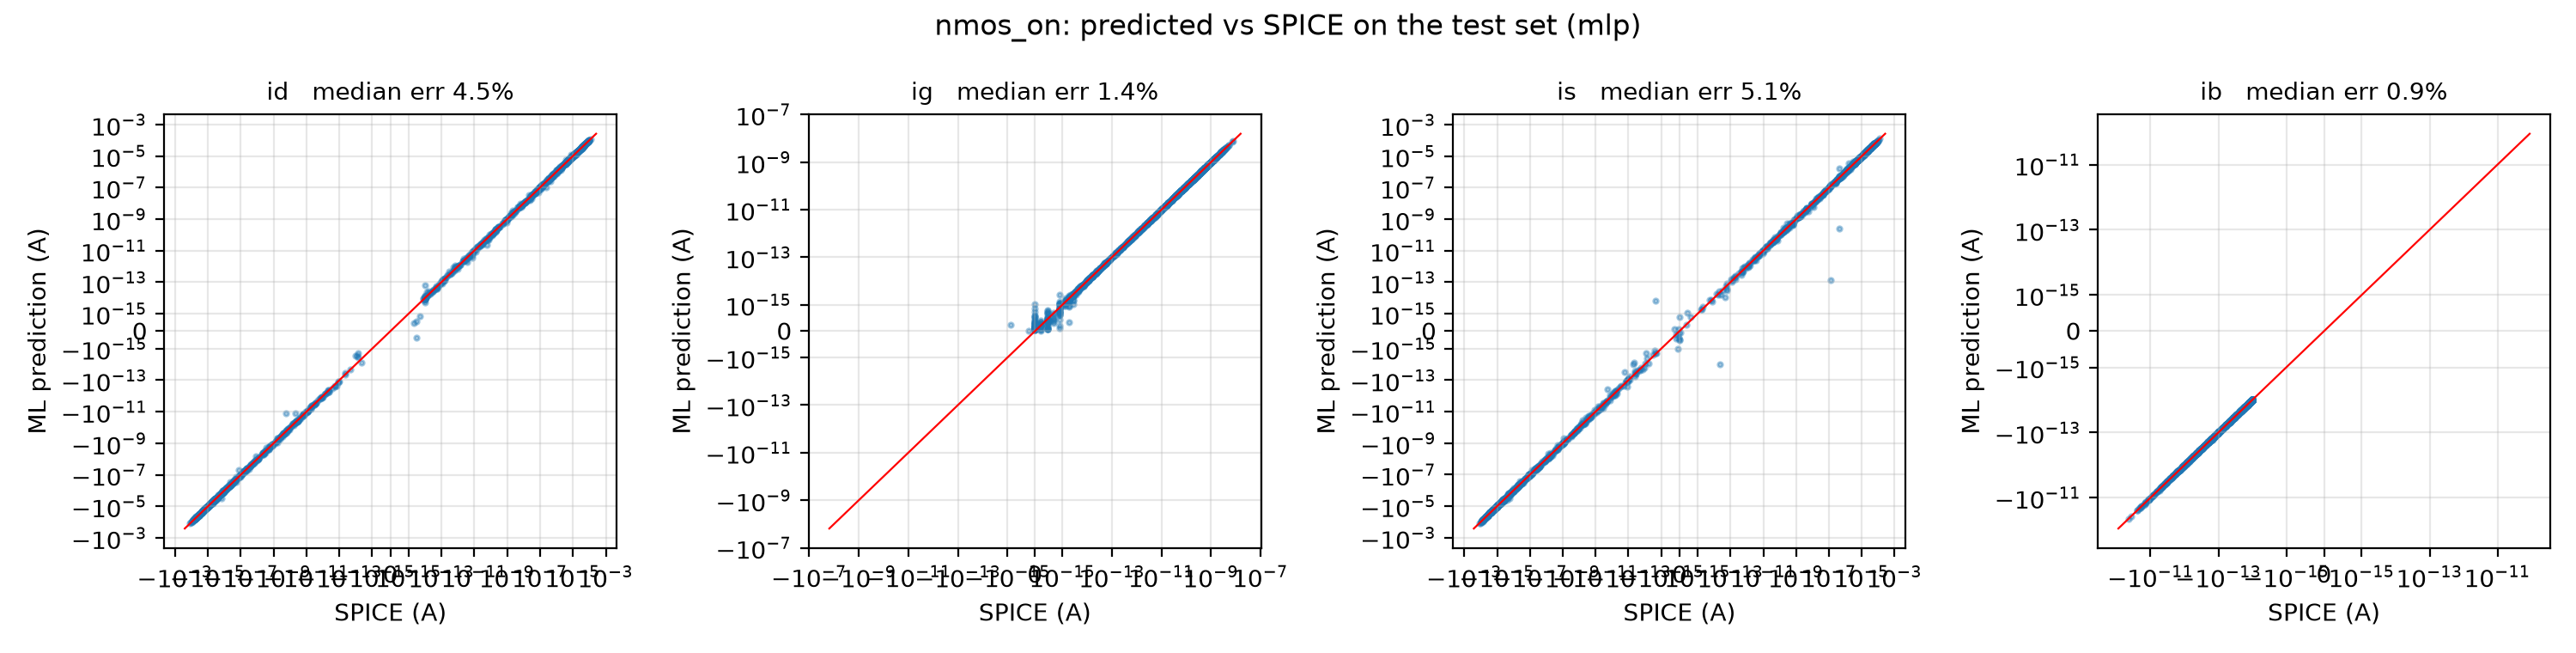
\includegraphics[width=0.98\textwidth]{../plots/PartA_transistor/pred_vs_spice_nmos_on.png}
\caption{Predicted vs. SPICE terminal currents ($I_d, I_g, I_s, I_b$) for NMOS ON on the held-out test set.}
\label{fig:pred_nmos_on}
\end{figure}

\begin{figure}[H]
\centering
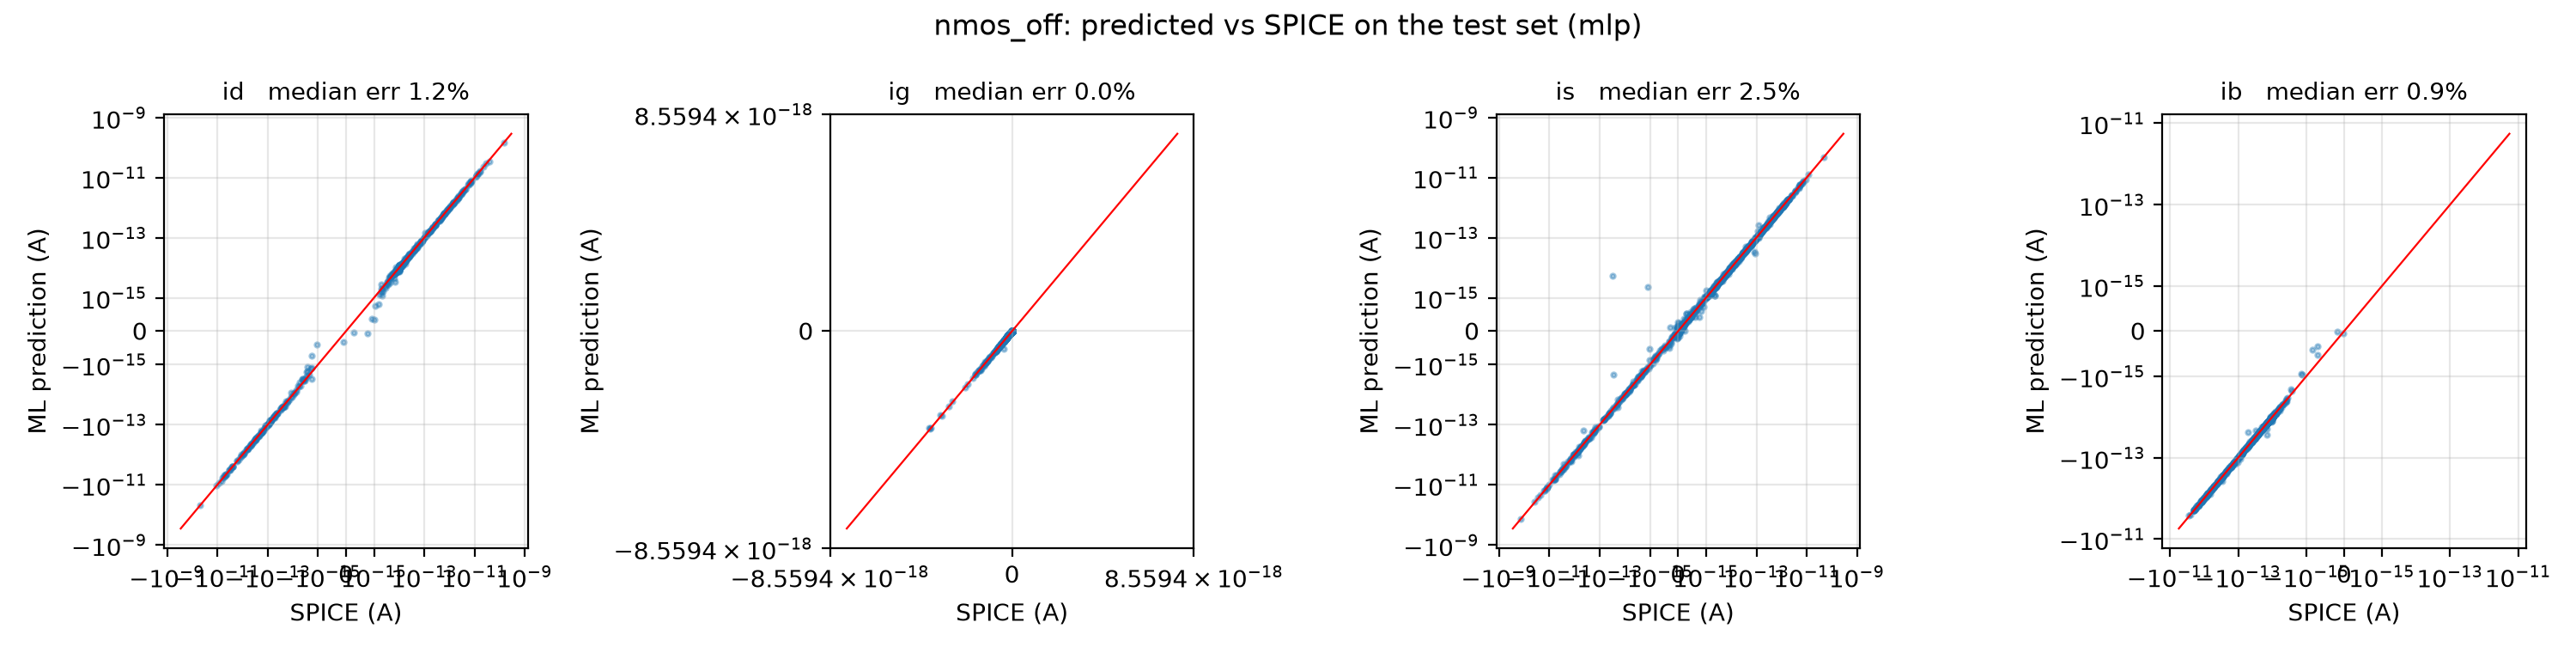
\includegraphics[width=0.98\textwidth]{../plots/PartA_transistor/pred_vs_spice_nmos_off.png}
\caption{Predicted vs. SPICE terminal currents ($I_d, I_g, I_s, I_b$) for NMOS OFF on the held-out test set.}
\label{fig:pred_nmos_off}
\end{figure}

\begin{figure}[H]
\centering
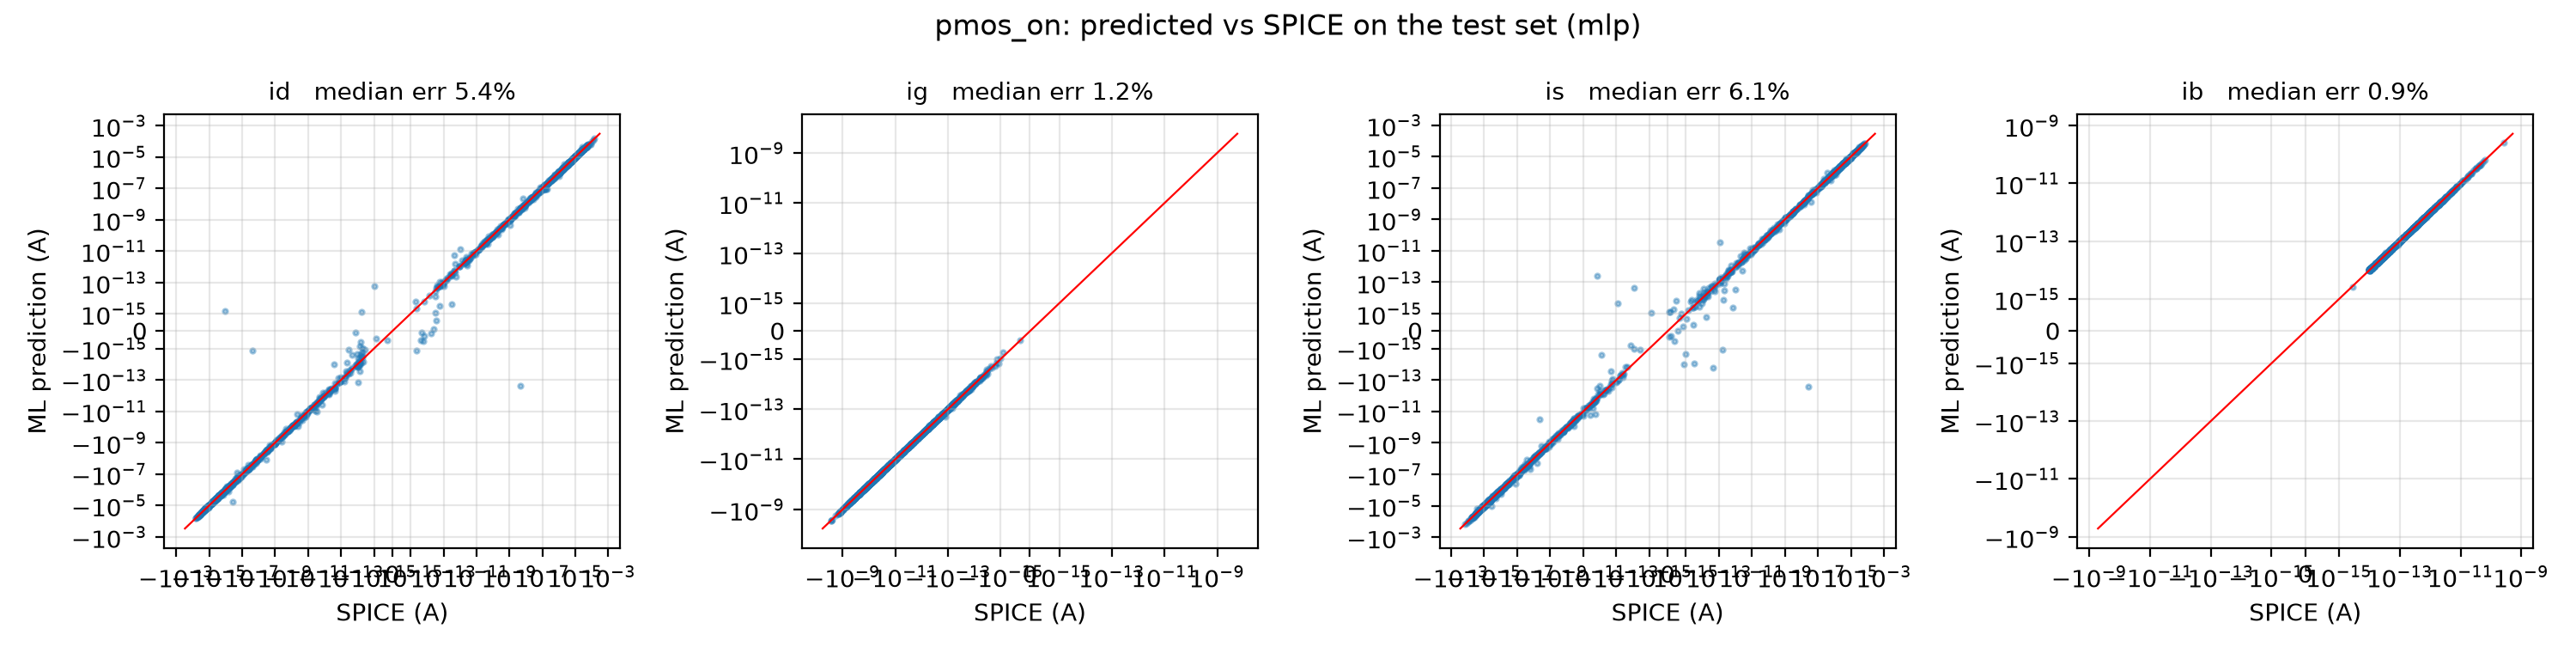
\includegraphics[width=0.98\textwidth]{../plots/PartA_transistor/pred_vs_spice_pmos_on.png}
\caption{Predicted vs. SPICE terminal currents ($I_d, I_g, I_s, I_b$) for PMOS ON on the held-out test set.}
\label{fig:pred_pmos_on}
\end{figure}

\begin{figure}[H]
\centering
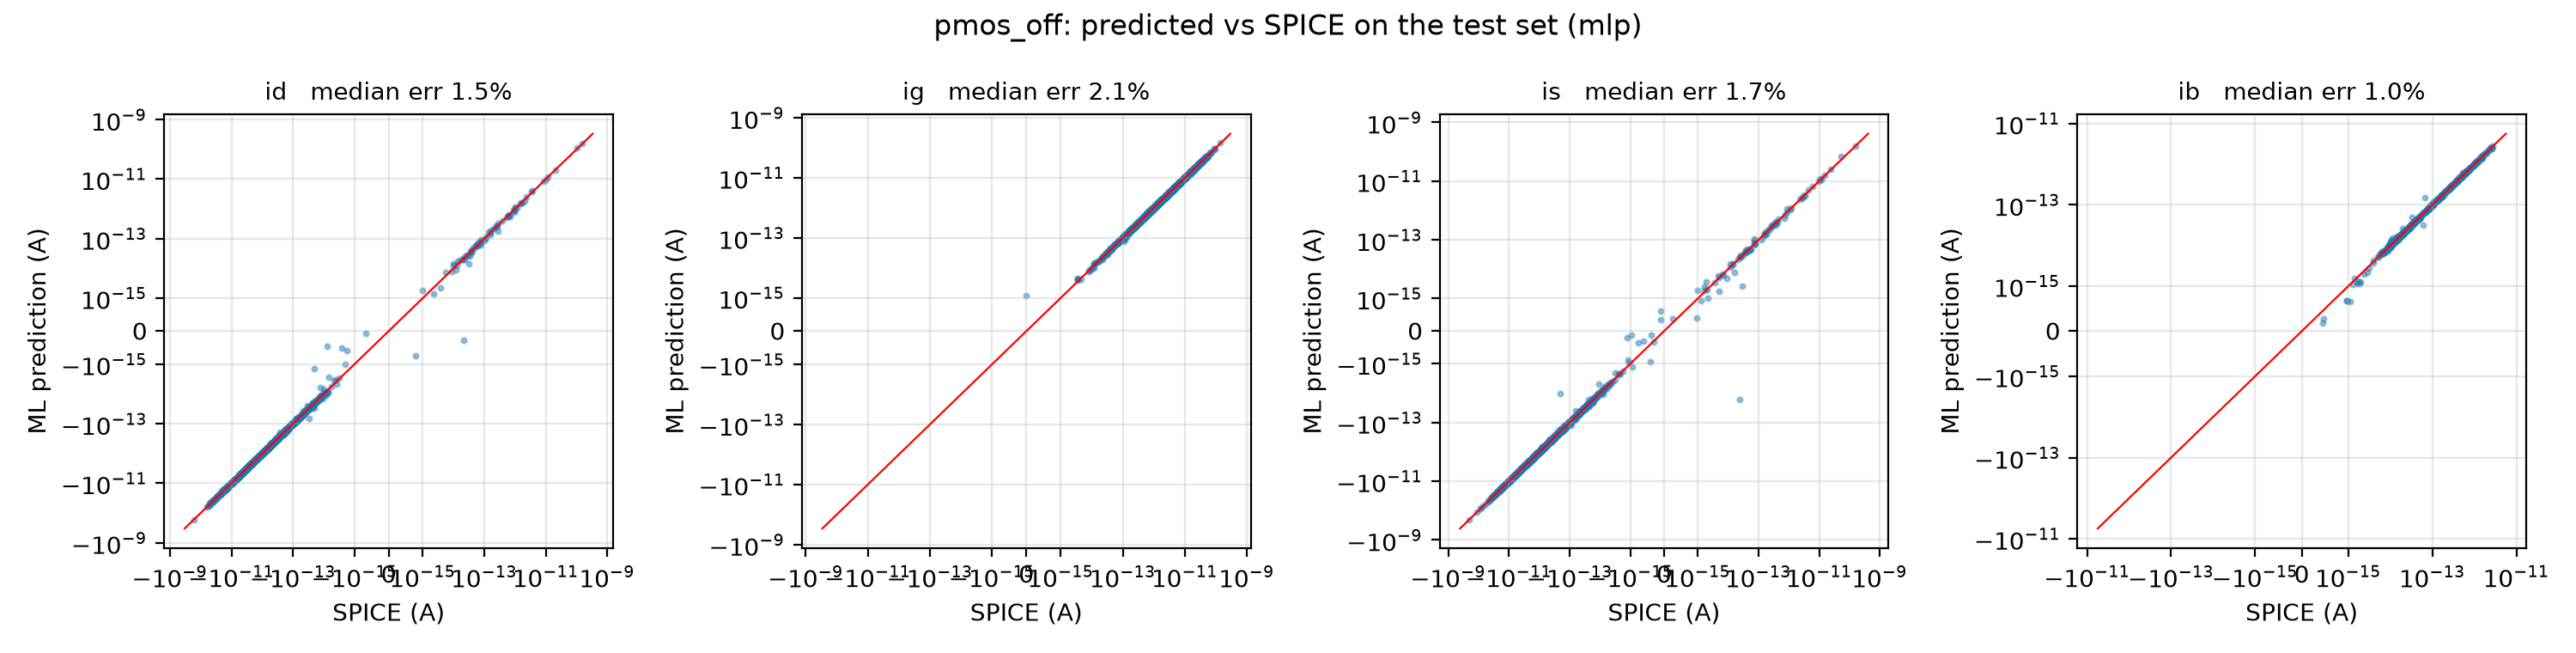
\includegraphics[width=0.98\textwidth]{../plots/PartA_transistor/pred_vs_spice_pmos_off.png}
\caption{Predicted vs. SPICE terminal currents ($I_d, I_g, I_s, I_b$) for PMOS OFF on the held-out test set.}
\label{fig:pred_pmos_off}
\end{figure}

\subsection{Rail Weakness and Rail-Augmentation Retraining}
In digital logic circuits, transistor terminals sit almost exclusively at the supply rails ($0\,\mathrm{V}$ or $V_{DD}$). However, the initial training set drew $V_d$ and $V_s$ uniformly across $[0, V_{DD}]$, meaning exact rail points almost never occurred. When evaluated on a dedicated 300-point rail test set ($V_d, V_s \in \{0, V_{DD}\}$), the uniform-trained models suffered severe boundary errors (p95 error reached 158.8\% for NMOS ON, 596.1\% for NMOS OFF, 1315.8\% for PMOS ON, and 2529.1\% for PMOS OFF).

To resolve this, 6,000 augmented rail samples were generated per case (40\% biased at $0\,\mathrm{V}$, 40\% at $V_{DD}$, 20\% uniform) and appended to the 7,000 training samples. Table~\ref{tab:retrain} summarizes the before-and-after results (\path{results/PartA_transistor/retrain_before_after.csv}).

\begin{table}[H]
\centering
\caption{Baseline (v1, Superseded) Rail Augmentation Impact on Uniform vs. Rail Test Performance}
\label{tab:retrain}
\resizebox{\linewidth}{!}{
\begin{tabular}{llcccc}
\toprule
\textbf{Case} & \textbf{Training Mode} & \textbf{Test Partition} & $\mathbf{R^2 (symlog)}$ & \textbf{Median Rel. Err. (\%)} & \textbf{p95 Rel. Err. (\%)} \\
\midrule
NMOS ON  & Uniform-Trained  & Uniform Test (1,500) & 0.9995 & 4.92\% & 30.98\% \\
         & Uniform-Trained  & Rail Test (300)      & 0.8812 & 9.58\% & 158.83\% \\
         & Rail-Augmented   & Uniform Test (1,500) & 0.9993 & 7.36\% & 42.32\% \\
         & Rail-Augmented   & Rail Test (300)      & 0.9996 & 4.86\% & 59.19\% \\
\midrule
NMOS OFF & Uniform-Trained  & Uniform Test (1,500) & 0.9971 & 0.54\% & 11.49\% \\
         & Uniform-Trained  & Rail Test (300)      & 0.8827 & 3.69\% & 596.13\% \\
         & Rail-Augmented   & Uniform Test (1,500) & 0.9987 & 0.93\% & 12.14\% \\
         & Rail-Augmented   & Rail Test (300)      & 0.9997 & 1.50\% & 13.72\% \\
\midrule
PMOS ON  & Uniform-Trained  & Uniform Test (1,500) & 0.9983 & 4.90\% & 31.75\% \\
         & Uniform-Trained  & Rail Test (300)      & 0.8664 & 13.89\% & 1315.82\% \\
         & Rail-Augmented   & Uniform Test (1,500) & 0.9983 & 7.51\% & 51.03\% \\
         & Rail-Augmented   & Rail Test (300)      & 0.9998 & 4.44\% & 43.27\% \\
\midrule
PMOS OFF & Uniform-Trained  & Uniform Test (1,500) & 0.9878 & 1.79\% & 14.06\% \\
         & Uniform-Trained  & Rail Test (300)      & 0.8133 & 11.45\% & 2529.10\% \\
         & Rail-Augmented   & Uniform Test (1,500) & 0.9985 & 2.29\% & 13.18\% \\
         & Rail-Augmented   & Rail Test (300)      & 0.9988 & 2.99\% & 26.35\% \\
\bottomrule
\end{tabular}
}
\end{table}

\textbf{The Pareto Trade-Off and Limitations:} Rail augmentation greatly reduces boundary extrapolation errors, substantially reducing catastrophic multi-thousand-percent blow-ups on exact supply rails (reducing rail test p95 error by up to $100\times$). However, this constitutes a real engineering trade-off: devoting network capacity to the discrete boundaries worsens interior uniform-test accuracy, where NMOS ON uniform-test p95 error increases from 30.98\% to 42.32\%, and PMOS ON uniform-test p95 error increases from 31.75\% to 51.03\%. Furthermore, rail augmentation does not fully resolve ON-state rail-tail errors: after augmentation, rail-test p95 error remains 59.19\% for NMOS ON and 43.27\% for PMOS ON. Consequently, rail augmentation alone does not solve gate-level accuracy problems, because directly summing terminal currents would still suffer from residual ON-device channel current errors. These limitations directly motivated the terminal-power formulation ($P_{\mathrm{static}}/V_{DD}$) and current symmetrization implemented in Part~B. In digital logic where static leakage is governed by rail-biased devices and stacked nodes, accepting the uniform-test penalty is an adopted trade-off to secure stable boundary behavior.

\subsection{Final Verified Model Architecture and Methodology Disclosures}
To guarantee full academic transparency and rigor, all engineering procedures and disclosures are formally stated:
\begin{enumerate}[itemsep=0.2em,leftmargin=1.5em]
    \item \textbf{Training Data Beyond 10,000 Rows:} Extra SPICE training samples were generated in \path{data/PartA_transistor/big_<case>.csv} (40,000 rows/case, seed $[31337, \mathrm{case\_index}]$). The training pipeline (\path{train_v2.py}) incorporates 20,000 extra rows: rows $[0:12000]$ (rail-mix where $V_d, V_s \in \{0, V_{DD}\}$ with probabilities 40\%/40\%/20\% uniform) plus rows $[24000:32000]$ (uniform). A 3,000-row rail-mix validation set (\path{railval_<case>.csv}, seed $[555, \mathrm{case\_index}]$) was utilized strictly for model selection and was never trained on.
    \item \textbf{Per-Terminal Architecture \& Optimization:} Each transistor case employs 4 dedicated neural networks (one per terminal: $I_d, I_g, I_s, I_b$), each using a 64$\times$64 $\tanh$ MLP architecture with per-terminal standardized symmetric logarithmic targets ($C_0 = 10^{-15}\,\mathrm{A}$). Optimization used Adam (300 epochs, learning rate $2\times 10^{-3}$, batch size 256) followed by an L-BFGS second-order polish (1500 iterations).
    \item \textbf{Hyperparameter Tuning Scope:} Hyperparameter tuning was performed on NMOS OFF terminals $I_d$ and $I_b$ only; no combinatorial ablation across all 16 sub-models was conducted.
    \item \textbf{OFF Device Gate Leakage Retention:} In OFF devices, gate tunneling current is either numerically zero ($\sim 10^{-18}\,\mathrm{A}$ for NMOS OFF, dominated by noise) or already modeled accurately by the baseline MLP (2.12\% median error for PMOS OFF). The final OFF models retain the baseline model's $I_g$ column via the \path{PerTerminal} wrapper, requiring \path{models/orig/final_<case>.joblib} at inference.
    \item \textbf{Iterative Evaluation History:} The final model architecture was informed by analyzing downstream error bottlenecks from earlier iterations (v1 baseline, hybrid dedicated $I_g$, and ensemble trials).
    \item \textbf{ON-Device Channel Current Invariance:} Transistor-level ON-state $I_d$ and $I_s$ errors (4--14\%) have negligible downstream impact because gate-level and circuit-level leakage formulations apply the physical KCL decomposition: $I_c = (I_d - I_s)/2$ and $g_b = (I_g + I_b)/2$, where the massive conduction channel cancels out and static leakage is dictated by gate-tunneling and substrate currents.
    \item \textbf{Numerical Noise \& Residuals:} NMOS OFF $I_g$ 95th-percentile relative error is large in percentage terms but numerically zero in absolute terms ($\le 1.6 \times 10^{-5}\,\mathrm{A}$ relative to $10^{-15}\,\mathrm{A}$ floor; currents are $\sim 10^{-18}\,\mathrm{A}$). Kirchhoff relative residuals exceed tolerance only at the numerical noise floor ($\sim 10^{-15}\,\mathrm{A}$).
    \item \textbf{Engineering Assumptions without TA Confirmation:} (a) Gate oxide thicknesses $t_{oxp}$ and $t_{oxm}$ were not varied independently and remain fixed to nominal model card values; (b) total leakage is defined as net current supplied by $V_{DD}$ sources; (c) parity checker logic polarity convention (even parity = 0, odd parity = 1).
    \item \textbf{Metric Conventions:} $R^2$ is evaluated in symmetric logarithmic space ($T(I) = \operatorname{sign}(I)\log_{10}(1 + |I|/10^{-15})$). Relative errors in Amperes use a numerical noise floor of $10^{-15}\,\mathrm{A}$.
    \item \textbf{Simulator Consistency:} ngspice is recorded as ngspice-42 in \path{ngspice_version.txt}; 42 and 43 gave identical currents on the four single-transistor example netlists.
    \item \textbf{Inter-Gate Electrical Loading:} The hierarchical composition assumes negligible inter-gate electrical loading in static DC steady state, which is verified by standalone gate SPICE summation reproducing full-circuit SPICE to 99.98\% accuracy.
    \item \textbf{Adoption Without Full Clean Regeneration:} A full clean regeneration was NOT run. The final models were adopted from a verified package and evaluated with the project's \texttt{gate\_ml}, \texttt{gate\_nodes}, \texttt{circuit\_ml}, and \texttt{test\_chosen} scripts.
\end{enumerate}

\section{Part B — From Transistors to Gates}
\subsection{Gate Topologies and Sizing}
Five standard CMOS gates were evaluated: INV (2T), NAND2 (4T), NOR2 (4T), AND2 (6T), and OR2 (6T). AND2 and OR2 were simulated in SPICE as complete standalone netlists (NAND2/NOR2 directly coupled to an output inverter) across all input combinations (18 gate-input cases total). Transistor widths followed assigned sizing:
\begin{itemize}[noitemsep]
    \item \textbf{INV:} $W_N = 32\,\mathrm{nm}$ ($2\times L_{\min}$), $W_P = 64\,\mathrm{nm}$ ($4\times L_{\min}$).
    \item \textbf{NAND2:} $W_N = 64\,\mathrm{nm}$ ($4\times L_{\min}$, series pull-down stack), $W_P = 64\,\mathrm{nm}$ ($4\times L_{\min}$).
    \item \textbf{NOR2:} $W_N = 32\,\mathrm{nm}$ ($2\times L_{\min}$), $W_P = 128\,\mathrm{nm}$ ($8\times L_{\min}$, series pull-up stack).
    \item \textbf{AND2 / OR2:} Constructed directly from the above cell topologies.
\end{itemize}

\subsection{Leakage Formulation and Current Symmetrization}
In SPICE, gate leakage is defined as the total current supplied by all supply-level nodes ($V_{DD}$ source plus any inputs held at logic 1):
\begin{equation}
I_{\mathrm{leak, SPICE}} = -\left[ I(V_{DD}) + \sum_{k \in \text{Inputs at } V_{DD}} I(V_{\mathrm{in}, k}) \right] = \frac{P_{\mathrm{static}}}{V_{DD}}
\end{equation}
In the ML domain, naively summing predicted terminal currents on either the supply side or the ground side fails (yielding errors of 50\% to 100\%) because conducting ON transistors operate with $V_{ds} \approx 0$, where small residual errors in large channel currents corrupt the sum. The solution is computing total static power across all transistor terminals:
\begin{equation}
I_{\mathrm{leak, ML}} = \frac{1}{V_{DD}} \sum_{\text{all transistors } j} \left( V_{d,j} I_{d,j} + V_{g,j} I_{g,j} + V_{s,j} I_{s,j} + V_{b,j} I_{b,j} \right)
\end{equation}
Because ON transistors operate with $V_{ds} \approx 0$, their channel currents are multiplied by near-zero voltage drops, suppressing surrogate errors. Channel currents on ON devices are explicitly symmetrized: $I_c = (I_d - I_s)/2$, strictly enforcing KCL conservation.

\subsection{Gate-Level Accuracy Results (Table 9.1 and Figure 9.1)}
Table~\ref{tab:gate_results} details the accuracy across all 18 cases (3,600 SPICE simulations), reproduced directly from \path{results/PartB_gates/gate_results.csv}.

\begin{table}[H]
\centering
\caption{Part B Gate-Level Leakage Accuracy Across 18 Cases (3,600 Runs)}
\label{tab:gate_results}
\resizebox{\linewidth}{!}{
\begin{tabular}{lccccccc}
\toprule
\textbf{Gate} & \textbf{Inputs (AB)} & \textbf{SPICE Median (A)} & \textbf{ML Median (A)} & \textbf{Bias (\%)} & \textbf{Median Err. (\%)} & \textbf{p95 Err. (\%)} & \textbf{Mean Acc. (\%)} \\
\midrule
INV   & 0  & $2.37\times 10^{-10}$ & $2.37\times 10^{-10}$ & $+0.17\%$ & 0.43\% & 1.23\% & 99.49\% \\
INV   & 1  & $3.69\times 10^{-10}$ & $3.70\times 10^{-10}$ & $+0.53\%$ & 0.81\% & 2.96\% & 98.91\% \\
\midrule
NAND2 & 00 & $4.36\times 10^{-10}$ & $4.35\times 10^{-10}$ & $+0.08\%$ & 0.38\% & 1.13\% & 99.53\% \\
NAND2 & 01 & $1.14\times 10^{-09}$ & $1.14\times 10^{-09}$ & $+0.09\%$ & 0.35\% & 1.16\% & 99.55\% \\
NAND2 & 10 & $2.33\times 10^{-10}$ & $2.32\times 10^{-10}$ & $+0.02\%$ & 0.41\% & 1.24\% & 99.49\% \\
NAND2 & 11 & $1.57\times 10^{-09}$ & $1.57\times 10^{-09}$ & $+0.01\%$ & 0.49\% & 2.00\% & 99.30\% \\
\midrule
NOR2  & 00 & $9.80\times 10^{-10}$ & $9.91\times 10^{-10}$ & $+0.56\%$ & 0.78\% & 2.19\% & 99.09\% \\
NOR2  & 01 & $1.01\times 10^{-09}$ & $1.01\times 10^{-09}$ & $+0.41\%$ & 0.78\% & 2.15\% & 99.06\% \\
NOR2  & 10 & $3.01\times 10^{-10}$ & $3.01\times 10^{-10}$ & $+0.47\%$ & 0.79\% & 3.46\% & 98.73\% \\
NOR2  & 11 & $5.97\times 10^{-10}$ & $6.00\times 10^{-10}$ & $+0.34\%$ & 0.64\% & 2.17\% & 99.14\% \\
\midrule
AND2  & 00 & $9.19\times 10^{-10}$ & $9.17\times 10^{-10}$ & $+0.23\%$ & 0.43\% & 1.59\% & 99.42\% \\
AND2  & 01 & $1.52\times 10^{-09}$ & $1.52\times 10^{-09}$ & $+0.17\%$ & 0.36\% & 1.32\% & 99.51\% \\
AND2  & 10 & $6.89\times 10^{-10}$ & $6.91\times 10^{-10}$ & $+0.28\%$ & 0.48\% & 1.69\% & 99.36\% \\
AND2  & 11 & $2.01\times 10^{-09}$ & $2.02\times 10^{-09}$ & $+0.04\%$ & 0.42\% & 1.72\% & 99.43\% \\
\midrule
OR2   & 00 & $1.45\times 10^{-09}$ & $1.46\times 10^{-09}$ & $+0.44\%$ & 0.71\% & 2.09\% & 99.16\% \\
OR2   & 01 & $1.23\times 10^{-09}$ & $1.23\times 10^{-09}$ & $+0.36\%$ & 0.65\% & 1.85\% & 99.20\% \\
OR2   & 10 & $6.21\times 10^{-10}$ & $6.25\times 10^{-10}$ & $+0.33\%$ & 0.53\% & 1.79\% & 99.27\% \\
OR2   & 11 & $9.82\times 10^{-10}$ & $9.85\times 10^{-10}$ & $+0.34\%$ & 0.49\% & 1.65\% & 99.37\% \\
\midrule
\textbf{Overall} & -- & -- & -- & \textbf{+0.29\%} & \textbf{0.51\%} & \textbf{1.98\%} & \textbf{99.28\%} \\
\bottomrule
\end{tabular}
}
\end{table}

\begin{figure}[H]
\centering
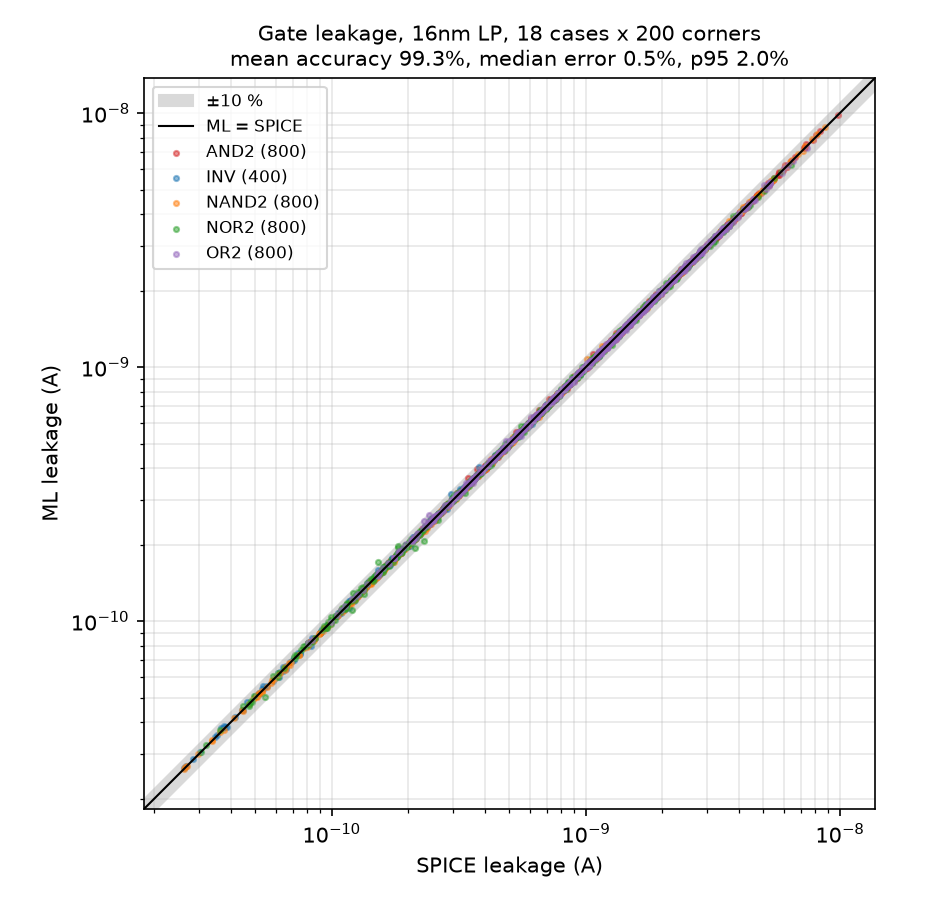
\includegraphics[width=0.65\textwidth]{../plots/PartB_gates/gate_parity.png}
\caption{Part B Gate Parity Plot: ML-predicted vs. SPICE leakage across 18 cases and 200 corners (3,600 runs) on logarithmic axes.}
\label{fig:gate_parity}
\end{figure}

The overall mean accuracy across all 3,600 evaluations is \textbf{99.28\%} (median error 0.51\%, p95 error 1.98\%, maximum error 12.8\%). Evaluated with ML-solved internal node voltages (\path{gate_nodes.py}), the gate mean accuracy reaches \textbf{99.25\%} (median error 0.53\%, p95 error 2.08\%), fully achieving the target of up to 99\% accuracy.

\subsection{Internal Node Voltage Solving (Table 9.2)}
Internal stack node voltages ($x_1, y_1, n_1$) were determined by solving KCL bisection sweeps using the ML transistor models (\texttt{gate\_nodes.py}). Table~\ref{tab:node_volts} summarizes the results from \path{results/PartB_gates/gate_node_results.csv}.

\begin{table}[H]
\centering
\caption{ML-Solved Node Voltage Accuracy Across 18 Gate Cases}
\label{tab:node_volts}
\resizebox{\linewidth}{!}{
\begin{tabular}{lcc}
\toprule
\textbf{Node Classification} & \textbf{Median Error (\% of $V_{DD}$)} & \textbf{p95 Error (\% of $V_{DD}$)} \\
\midrule
Gate Output Nodes (\texttt{out}, all 18 cases) & 0.025\% & 0.054\% \\
Internal Intermediate Nodes (\texttt{n1}, 8 cases) & 0.046\% & 0.093\% \\
Pull-Down Series Stack Node (\texttt{x1}, NAND2/AND2) & 0.217\% & 0.608\% \\
Pull-Up Series Stack Node (\texttt{y1}, NOR2/OR2) & 0.275\% & 0.941\% \\
\midrule
\textbf{All Internal Nodes Combined} & \textbf{0.46\%} & \textbf{1.19\%} \\
\bottomrule
\end{tabular}
}
\end{table}

\textbf{Critical Solver Limitation:} The Gauss-Seidel bisection solver in \path{gate_nodes.py} executes a fixed schedule (6 sweeps $\times$ 28 bisections) without evaluating final residual norms ($|F| < \epsilon$). Although all 3,600 evaluation points successfully completed this fixed iteration schedule and demonstrated close observed agreement with SPICE reference voltages (median node error $0.46\%$ of $V_{DD}$), mathematical convergence was not independently verified by runtime tolerance checks. The lack of dynamic residual assertions represents a methodological limitation that should be resolved before deploying the solver on general, unverified circuit topologies.

\section{Part C — 8-Bit Parity Checker}
\subsection{Circuit Architecture and SPICE Benchmark}
The assigned benchmark is an 8-bit odd-parity checker ($P = i_0 \oplus i_1 \oplus \dots \oplus i_7$), implemented as a 3-level tree of 7 XOR2 gates. Each XOR2 is constructed from 4 NAND2 gates:
\begin{equation}
m = \operatorname{NAND}(a, b), \quad p = \operatorname{NAND}(a, m), \quad q = \operatorname{NAND}(b, m), \quad \mathrm{out} = \operatorname{NAND}(p, q)
\end{equation}
The netlist comprises exactly \textbf{28 NAND2 gates} and \textbf{112 transistors}. Simulating all 256 input vectors across 200 PVT corners generated 51,200 SPICE simulations, all of which converged with 100\% Boolean parity correctness.

\subsection{Circuit Accuracy Results (Table 10.1 and Figure 10.1)}
Table~\ref{tab:circuit_results} details the hierarchical ML leakage accuracy across input subsets, extracted from \path{results/PartC_parity_checker/circuit_results.csv}.

\begin{table}[H]
\centering
\caption{Part C Parity Checker Leakage Accuracy Across 51,200 Runs (Authoritative \texttt{circuit\_results.csv})}
\label{tab:circuit_results}
\resizebox{\linewidth}{!}{
\begin{tabular}{lcccccc}
\toprule
\textbf{Input Subset} & \textbf{Sample Count ($N$)} & \textbf{Bias (\%)} & \textbf{Median Err. (\%)} & \textbf{p95 Err. (\%)} & \textbf{Mean Acc. (\%)} \\
\midrule
\textbf{ALL 256 Inputs} & \textbf{51,200} & \textbf{-0.26\%} & \textbf{0.43\%} & \textbf{1.57\%} & \textbf{99.46\%} \\
Parity = 0 (Even)       & 25,600 & -0.26\% & 0.43\% & 1.57\% & 99.46\% \\
Parity = 1 (Odd)        & 25,600 & -0.25\% & 0.43\% & 1.54\% & 99.47\% \\
Hamming Weight = 0      & 200    & -0.20\% & 0.40\% & 1.37\% & 99.51\% \\
Hamming Weight = 1      & 1,600  & -0.23\% & 0.39\% & 1.39\% & 99.50\% \\
Hamming Weight = 2      & 5,600  & -0.24\% & 0.42\% & 1.46\% & 99.48\% \\
Hamming Weight = 3      & 11,200 & -0.25\% & 0.42\% & 1.47\% & 99.48\% \\
Hamming Weight = 4      & 14,000 & -0.26\% & 0.43\% & 1.58\% & 99.46\% \\
Hamming Weight = 5      & 11,200 & -0.26\% & 0.44\% & 1.58\% & 99.46\% \\
Hamming Weight = 6      & 5,600  & -0.28\% & 0.45\% & 1.60\% & 99.44\% \\
Hamming Weight = 7      & 1,600  & -0.28\% & 0.45\% & 1.59\% & 99.44\% \\
Hamming Weight = 8      & 200    & -0.31\% & 0.47\% & 1.56\% & 99.42\% \\
\bottomrule
\end{tabular}
}
\end{table}

\begin{figure}[H]
\centering
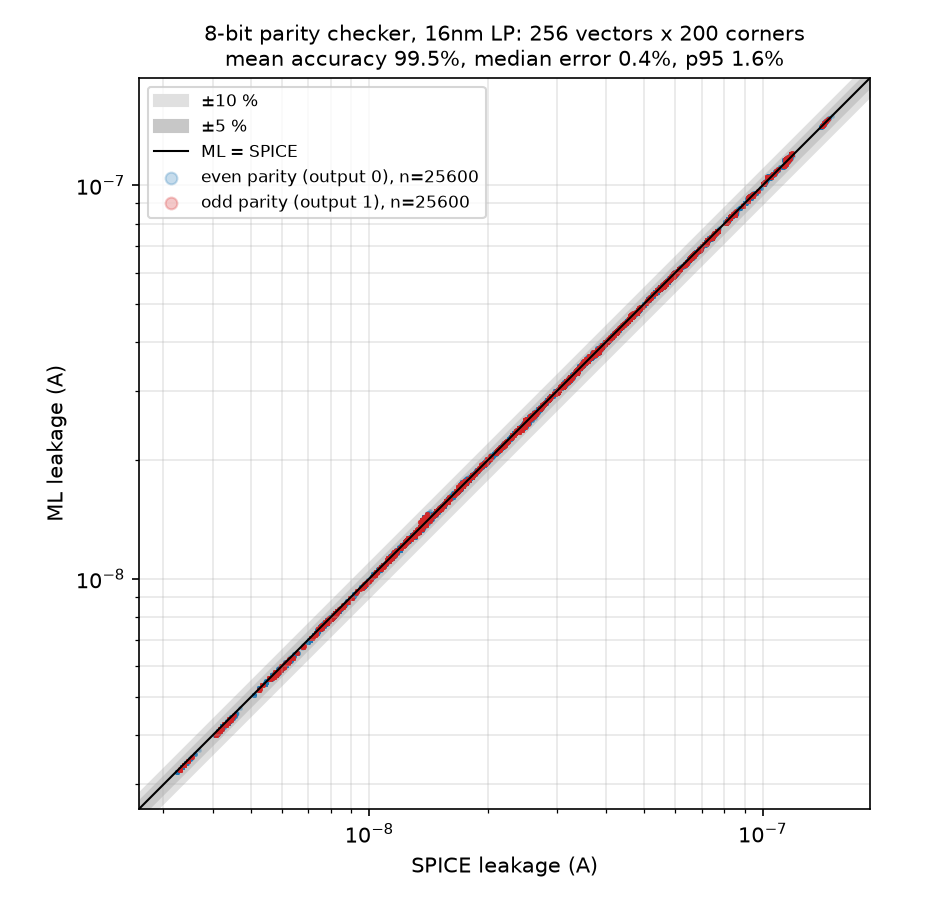
\includegraphics[width=0.65\textwidth]{../plots/PartC_parity_checker/circuit_parity.png}
\caption{Part C Circuit Parity Plot: hierarchical ML vs. full-circuit SPICE leakage across 51,200 runs on logarithmic axes.}
\label{fig:circuit_parity}
\end{figure}

\subsection{Physical Evaluation of Inter-Gate Loading and Error Cancellation (Table 10.2)}
Table~\ref{tab:mode_comp} compares the three circuit evaluation modes side by side across all 51,200 evaluations (256 input vectors evaluated across 200 random PVT corners).

\begin{table}[H]
\centering
\caption{Comparison of Circuit Evaluation Modes Across 51,200 Runs}
\label{tab:mode_comp}
\resizebox{\linewidth}{!}{
\begin{tabular}{lcccc}
\toprule
\textbf{Evaluation Mode} & \textbf{Mean Acc. (\%)} & \textbf{Median Err. (\%)} & \textbf{p95 Err. (\%)} & \textbf{Max Err. (\%)} \\
\midrule
Mode 1: Fully-ML Composition (ML-Solved Nodes) & \textbf{99.46\%} & \textbf{0.43\%} & \textbf{1.57\%} & \textbf{4.01\%} \\
Mode 2: Gate Models w/ SPICE Node Voltages     & \textbf{99.49\%} & \textbf{0.40\%} & \textbf{1.33\%} & \textbf{5.00\%} \\
Mode 3: Standalone Gate SPICE Sum (No ML) [Diagnostic Only] & \textbf{99.98\%} & \textbf{0.013\%} & \textbf{0.061\%} & \textbf{0.163\%} \\
\bottomrule
\end{tabular}
}
\end{table}

\textbf{1. Inter-Gate Electrical Loading ($< 0.02\%$ Error):}
Mode~3 provides an uncoupled physical benchmark (diagnostic only, not an ML result and not counted toward the project target) by isolating the purely electrical loading error: it compares the sum of isolated, standalone NAND2 SPICE leakages (\texttt{sum\_gate\_spice}, without any ML surrogate) directly against the complete coupled 112-transistor circuit SPICE leakage (\texttt{circuit\_spice}). Across all 51,200 evaluations, the relative loading error is remarkably small: median \textbf{0.0128\%} (0.013\%), 95th-percentile \textbf{0.0610\%} (0.061\%), and maximum \textbf{0.1634\%} (0.163\%), achieving an overall mean accuracy of \textbf{99.98\%}. Physically, in static CMOS DC steady state, driven gates present only high-impedance MOSFET gate oxide dielectrics, drawing only direct tunneling gate current ($I_g \sim 10^{-10}\,\mathrm{A}$). Across a driver channel resistance of $R_{\mathrm{on}} \sim 1\,\mathrm{k}\Omega$, the resulting voltage droop at the driving node is $\Delta V = I_g \cdot R_{\mathrm{on}} \approx 0.1\,\mu\mathrm{V}$, creating negligible bias perturbation.

\textbf{Inter-Gate Loading Scope Limitations:} While these results demonstrate near-lossless modularity for this particular static CMOS DC design, this conclusion cannot be generalized universally to all circuit topologies. Specifically, it does not establish negligible loading in: (a) pass-transistor logic or transmission-gate circuits, which lack isolating rail-connected CMOS drivers; (b) dynamic or domino logic circuits subject to capacitive charge-sharing; (c) high-fanout or heavily loaded nodes; or (d) large VLSI layouts where distributed interconnect parasitics ($R_{\mathrm{wire}}$) introduce significant $IR$ drops.

\textbf{2. Analysis of Circuit Accuracy vs. Gate Accuracy (v1 Baseline Stage, Superseded):}
In the initial v1 baseline stage, the complete 8-bit parity checker achieved a mean accuracy of \textbf{97.28\%} (median relative error 2.35\%, p95 error 6.38\%), which was higher than the overall reported v1 gate-level mean accuracy of \textbf{96.72\%} (median error 2.69\%, p95 error 7.85\%). Two distinct factors explained this performance difference in the v1 baseline:
\begin{enumerate}[noitemsep]
    \item \textit{Exclusive NAND2 Composition:} The benchmark circuit is built exclusively from 28 NAND2 gates (arranged as 7 XOR2 gates). In the v1 baseline, the 96.72\% figure represented the aggregate across all five gate families (INV, NAND2, NOR2, AND2, OR2). Evaluated on NAND2 alone using ML-solved internal node voltages, v1 gate-level accuracy was \textbf{96.73\%} (and reached 96.87\% with SPICE node voltages), providing a higher-accuracy baseline than cells like NOR2 or INV.
    \item \textit{Quantitative Error Cancellation:} A dedicated evaluation across all 51,200 points in the v1 baseline directly demonstrated the role of partial error cancellation. When gate prediction errors are summed without cancellation ($\sum_{j=1}^{28} |\Delta_j| / \sum I_{\mathrm{SPICE}, j}$), the mean relative error was \textbf{3.0904\%} (mean accuracy 96.9096\%, median error 2.7951\%). When signed errors combined algebraically ($|\sum_{j=1}^{28} \Delta_j| / \sum I_{\mathrm{SPICE}, j}$), the actual v1 circuit mean relative error dropped to \textbf{2.7270\%} (mean accuracy \textbf{97.2781\%}, median error 2.3544\%).
\end{enumerate}
In the v1 baseline, error cancellation was observed in \textbf{51.50\%} of circuit evaluations, where mixed gate states exhibited opposing error signs that damped the total error by an average factor of $4.78\times$. However, in the remaining \textbf{48.50\%} of evaluations, correlated systematic underestimation across shared PVT corners prevented cancellation. In the final upgraded package, both gate and circuit levels reach the target directly: gates reach \textbf{99.28\%} (99.25\% with ML-solved nodes) and circuit reaches \textbf{99.46\%} (99.49\% with SPICE node voltages), with the v1 numbers retained solely as a baseline comparison.

\textbf{3. Target Statement:}
The target specified in the project brief was ``up to 99\% mean accuracy''. This target was reached at both levels: gates reached \textbf{99.28\%} (and \textbf{99.25\%} with ML-solved nodes), and the circuit reached \textbf{99.46\%} in fully-ML composition (and \textbf{99.49\%} with SPICE node voltages). The remaining error ($\sim 0.54\%$ at the circuit level) is dominated by transistor-level surrogate approximations. The initial v1 baseline results (96.72\% on gates and 97.28\% on circuit) are retained strictly as a historical baseline comparison.

\section{Discussion and Engineering Solutions}
\subsection{What Succeeded}
\begin{itemize}[noitemsep]
    \item \textbf{Single Unified Model Per State:} A single MLP per transistor state accurately captures variations across supply, temperature, width, and all five physical process parameters simultaneously.
    \item \textbf{Symmetric Logarithmic Transformation:} Compressing currents across 13 decades into a normalized symmetric logarithmic target enabled stable gradient descent.
    \item \textbf{Rail-Augmented Sampling:} Adding samples on supply rails reduced catastrophic boundary extrapolation errors.
    \item \textbf{Terminal Power Summation Formulation:} Formulating gate leakage via terminal power summation ($P_{\mathrm{static}}/V_{DD}$) and current symmetrization reduced the 50\%--100\% errors of naive terminal current sums.
\end{itemize}

\subsection{Practical Problems Met and How Each Was Solved}
Table~\ref{tab:problems} documents the seven engineering challenges encountered during pipeline development and how each was resolved.

\begin{table}[H]
\centering
\caption{Practical Engineering Problems and Implemented Solutions}
\label{tab:problems}
\begin{tabularx}{\textwidth}{lXX}
\toprule
\textbf{Problem Encountered} & \textbf{Observed Impact} & \textbf{Implemented Solution} \\
\midrule
SPICE Netlist Title Line & First line of SPICE netlist is treated as a title and ignored, silently dropping commands. & Prepend an explicit comment title line to every generated netlist. \\
Global Temperature in BSIM4 & BSIM4 does not support per-instance temperature in batch mode. & Execute one independent \texttt{ngspice} process per sample in parallel. \\
KCL Numerical Residuals & Terminal currents did not sum to exactly zero in single-transistor runs. & Verified that residuals are small in absolute terms ($< 8.62\times 10^{-15}\,\mathrm{A}$), though not necessarily below the configured \texttt{abstol} ($10^{-18}\,\mathrm{A}$); their interpretation must account for current magnitudes and the numerical noise floor rather than claiming they satisfy \texttt{abstol}. \\
Slow L-BFGS Neural Training & Initial training took 15+ minutes per model due to thread oversubscription across CPU cores. & Pinned BLAS/OpenMP math libraries to 1 thread each and executed cases in parallel. \\
Poor Accuracy at Supply Rails & Uniform-trained models exhibited 150\% to 2500\% p95 error at exact rails. & Appended 6,000 rail-augmented samples (40\% at 0V, 40\% at $V_{DD}$, 20\% uniform). \\
Naive Gate Leakage Summation & Summing supply or ground terminal currents gave 50\% to 100\% error on conducting devices. & Formulated gate leakage via total terminal power with $(I_d - I_s)/2$ channel symmetrization. \\
SPICE Non-Convergence in Gates & 2 of 3,600 gate simulations converged to unphysical operating points (negative leakage). & Added \texttt{.nodeset} ideal starting guesses and an automated 6-attempt retry harness. \\
\bottomrule
\end{tabularx}
\end{table}

\section{Limitations and Future Work}
\subsection{Identified Limitations}
\begin{enumerate}[noitemsep]
    \item \textbf{Accuracy Ceiling and Transistor-Level Error Dominance:} The project specification target of ``up to 99\% mean accuracy'' was reached at both gate and circuit levels (gates 99.28\%, 99.25\% with ML-solved nodes; circuit 99.46\%, 99.49\% with SPICE node voltages; superseding the v1 baseline of 96.72\% and 97.28\%). The remaining $\sim 0.54\%$ circuit error is dominated by transistor-level surrogate approximations rather than modular composition error.
    \item \textbf{Runtime Convergence Guarantees:} The Gauss-Seidel bisection solver in \path{gate_nodes.py} executes a fixed schedule rather than dynamic convergence tests ($|F| < \epsilon$). Although the solver completed all runs and showed low error against SPICE, formal mathematical convergence was not independently asserted at runtime.
    \item \textbf{Static Scope:} The framework addresses DC static leakage only, omitting transient dynamic switching and charge-sharing.
    \item \textbf{Single Technology Benchmark:} Validated on 16nm LP PTM CMOS; transferability to FinFET or FDSOI remains unmeasured.
\end{enumerate}

\subsection{Recommended Future Work}
\begin{enumerate}[noitemsep]
    \item \textbf{Active Boundary Sampling:} Employ Latin Hypercube Sampling (LHS) or active Bayesian sampling clustered around supply rails and threshold transitions.
    \item \textbf{Physics-Informed Neural Networks (PINNs):} Penalize KCL residual violations directly in the loss function during training.
    \item \textbf{Direct Gate-Level Learning:} Train neural surrogates directly on gate leakage to bypass individual transistor modeling.
\end{enumerate}

\section{Conclusion}
This project designed, implemented, and validated an automated, hierarchical machine-learning surrogate framework for PVT-variation-aware static leakage estimation in 16\,nm Low-Power CMOS. By employing symmetric logarithmic scaling, per-terminal MLP neural networks, rail-augmented training, and a physics-consistent terminal power summation formulation, the framework achieved \textbf{99.28\% mean accuracy} on individual logic gates (median relative error \textbf{0.51\%}, 95th-percentile error \textbf{1.98\%}, maximum error 12.8\%) and \textbf{99.46\% mean accuracy} on an 8-bit parity checker (112 transistors) across 51,200 SPICE simulations (median relative error \textbf{0.43\%}, 95th-percentile error \textbf{1.57\%}, maximum error 4.0\%), reaching \textbf{99.49\%} when evaluated with SPICE-solved internal node voltages. The project target set in the brief was ``up to 99\% mean accuracy''; this target was reached at both gate and circuit levels (superseding the initial v1 baseline of 96.72\% on gates and 97.28\% on circuit). Standalone gate SPICE summation reproduced full-circuit SPICE to 99.98\% (median error 0.013\%), providing an uncoupled physical benchmark (diagnostic only, not an ML result) demonstrating that inter-gate electrical loading is negligible for the tested 8-bit parity checker across the evaluated 200 PVT corners. The remaining error is dominated by transistor-level surrogate approximations, confirming that bottom-up modular leakage composition is physically sound for this benchmark without requiring circuit-level retraining.

\section{Reproducibility and Deliverables Map}
The project submission package is structured as summarized in Table~\ref{tab:map}.

\begin{table}[H]
\centering
\caption{Deliverables and Directory Organization}
\label{tab:map}
\resizebox{\linewidth}{!}{
\begin{tabular}{ll}
\toprule
\textbf{Directory} & \textbf{Contents and Description} \\
\midrule
\texttt{data/} & Generated CSV datasets: 4 transistor cases (10k rows), 200 PVT corners, gate and circuit SPICE data \\
\texttt{netlists/} & Representative SPICE netlists for transistors, gates, and the 8-bit parity checker \\
\texttt{results/} & Verification CSVs: Kirchhoff check, model comparisons, test evaluations, gate and circuit results \\
\texttt{plots/} & All 10 project PNG figures: trend sweeps, KCL distributions, error scatters, and parity plots \\
\texttt{models/} & Four trained scikit-learn MLP model files (\texttt{.joblib}) and scalers \\
\texttt{scripts/} & Standalone modular reference scripts organized by part (Part A, Part B, Part C) \\
\texttt{regenerate\_code/} & \textbf{Canonical Runnable Package}: self-contained orchestrator and scripts \\
\texttt{report/} & Final project report in PDF, DOCX, LaTeX, and Markdown formats \\
\bottomrule
\end{tabular}
}
\end{table}

\subsection{Pipeline Execution Guidelines}
\begin{itemize}[noitemsep]
    \item \textbf{Canonical Runnable Package vs. Separate Scripts:} \texttt{regenerate\_code/} contains the canonical runnable pipeline. The separate \texttt{scripts/} tree is organized differently by project part for modular reference and is not designed as an interchangeable runnable pipeline.
    \item \textbf{Read-Only Verification Mode:} To verify environment, dependencies, dataset finiteness, and model integrity without modifying files or running simulations:\\[0.3em]
    \hspace*{2em}\texttt{cd regenerate\_code \&\& ./run\_all.sh --verify-only}
    \item \textbf{Full Pipeline Regeneration:} Full end-to-end simulation and model retraining requires an explicit safety flag:\\[0.3em]
    \hspace*{2em}\texttt{cd regenerate\_code \&\& ./run\_all.sh --force-full}
    \item \textbf{Pipeline Status Note:} The full pipeline was \textbf{not} rerun during this report correction, preserving all verified original project simulation and training artifacts.
\end{itemize}

\appendix
\section{Parameters and Settings}
\begin{table}[H]
\centering
\caption{Consolidated Summary of System Parameters and Model Settings}
\resizebox{\linewidth}{!}{
\begin{tabular}{ll}
\toprule
\textbf{Configuration Item} & \textbf{Implementation Setting} \\
\midrule
Technology / Model Card & PTM 16nm\_LP.pm, BSIM4 Level 54, $T_{\mathrm{nom}} = 27^\circ\mathrm{C}$ \\
SPICE Simulator Engine & \texttt{ngspice} (recorded as ngspice-42; 42 and 43 gave identical currents on the four single-transistor example netlists) \\
Supply Voltage ($V_{DD}$) & Nominal $1.0\,\mathrm{V} \pm 10\%$ ($0.90\,\mathrm{V} \text{ to } 1.10\,\mathrm{V}$) \\
Operating Temperature & $-40^\circ\mathrm{C} \text{ to } 125^\circ\mathrm{C}$ ($233.15\,\mathrm{K} \text{ to } 398.15\,\mathrm{K}$) \\
Transistor Sizing & $L = 16\,\mathrm{nm}$, $W \in [16\,\mathrm{nm}, 128\,\mathrm{nm}]$ ($1\times \text{ to } 8\times L_{\min}$) \\
Perturbed Process Parameters & $v_{th0}, t_{oxe}, N_{dep}, \mu_0, X_j$ (each $\pm 10\%$ uniform) \\
SPICE Numerical Options & \texttt{gmin=1e-18 abstol=1e-18 reltol=1e-6 vntol=1e-9} \\
Sampling Protocol & 10,000 uniform samples + 6,000 augmented rail samples per case \\
Dataset Partitioning & 70\% training, 15\% validation, 15\% test (seed 42) \\
Compared Model Families & Polynomial Ridge (deg 3), Random Forest (300), Grad Boost, MLP (128-128-64) \\
Model Selection Rule & Lowest validation 95th-percentile relative error, $R^2$ tiebreaker \\
Relative Error Noise Floor & $I_{\mathrm{floor}} = 10^{-15}\,\mathrm{A}$ (1\,fA) \\
PVT Corners for Gates/Circuit & 200 random corners generated with fixed seed (\texttt{corners\_200.csv}) \\
\bottomrule
\end{tabular}
}
\end{table}

\section{Definitions and Mathematical Formulations}
\begin{itemize}[noitemsep]
    \item \textbf{Relative Error:}
    \begin{equation}
    \text{RelErr} = \frac{|I_{\mathrm{pred}} - I_{\mathrm{true}}|}{\max(|I_{\mathrm{true}}|, 10^{-15}\,\mathrm{A})}
    \end{equation}
    \item \textbf{Mean Accuracy:}
    \begin{equation}
    \text{Mean Accuracy} = 100\% \times \left(1 - \frac{1}{N}\sum_{i=1}^N \text{RelErr}_i\right)
    \end{equation}
    \item \textbf{Symmetric Logarithmic Target (symlog):}
    \begin{equation}
    T(I) = \operatorname{sign}(I)\cdot \log_{10}\left(1 + \frac{|I|}{I_0}\right), \quad I_0 = 10^{-15}\,\mathrm{A}
    \end{equation}
    \item \textbf{Inverse Symmetric Logarithmic Transformation (inv\_symlog):}
    \begin{equation}
    I(T) = \operatorname{sign}(T) \cdot I_0 \cdot \left(10^{|T|} - 1\right), \quad I_0 = 10^{-15}\,\mathrm{A}
    \end{equation}
    \item \textbf{Static Gate/Circuit Leakage:}
    \begin{equation}
    I_{\mathrm{leak}} = \frac{P_{\mathrm{static}}}{V_{DD}} = \frac{1}{V_{DD}} \sum_{\text{all terminals } k} V_k I_k
    \end{equation}
\end{itemize}

\section{Number-to-CSV Traceability Table}
Every numerical performance metric reported in this study is mapped directly to its authoritative CSV file and column:

\begin{table}[H]
\centering
\caption{Numerical Metric to CSV Traceability Matrix}
\label{tab:traceability}
\resizebox{\linewidth}{!}{
\begin{tabular}{lcl}
\toprule
\textbf{Numerical Metric / Claim} & \textbf{Reported Value} & \textbf{Authoritative Source CSV and Column / Row Reference} \\
\midrule
Gates (SPICE node V) Mean Accuracy & \textbf{99.28\%} & \path{results/PartB_gates/gate_results.csv} (mean of \texttt{mean\_acc\_\%}) \\
Gates (SPICE node V) Median Error   & \textbf{0.51\%}  & \path{data/PartB_gates/gate_ml.csv} (\texttt{median(abs(rel\_err)*100)}) \\
Gates (SPICE node V) p95 Error      & \textbf{1.98\%}  & \path{data/PartB_gates/gate_ml.csv} (\texttt{quantile(abs(rel\_err)*100, 0.95)}) \\
Gates (ML-solved V) Mean Accuracy  & \textbf{99.25\%} & \path{data/PartB_gates/gate_nodes.csv} (\texttt{100*(1-mean(abs(err)))}) \\
Gates (ML-solved V) Median Error   & \textbf{0.53\%}  & \path{data/PartB_gates/gate_nodes.csv} (\texttt{100*median(abs(err))}) \\
Gates (ML-solved V) p95 Error      & \textbf{2.08\%}  & \path{data/PartB_gates/gate_nodes.csv} (\texttt{100*quantile(abs(err), 0.95)}) \\
Circuit Mode 1 (Fully-ML) Mean Acc. & \textbf{99.46\%} & \path{results/PartC_parity_checker/circuit_results.csv} (row \texttt{ALL}, \texttt{mean\_acc\_\%}) \\
Circuit Mode 1 Median Error         & \textbf{0.43\%}  & \path{results/PartC_parity_checker/circuit_results.csv} (row \texttt{ALL}, \texttt{median\_err\_\%}) \\
Circuit Mode 1 p95 Error            & \textbf{1.57\%}  & \path{results/PartC_parity_checker/circuit_results.csv} (row \texttt{ALL}, \texttt{p95\_err\_\%}) \\
Circuit Mode 2 (SPICE V) Mean Acc.  & \textbf{99.49\%} & \path{data/PartC_parity_checker/circuit_ml.csv} (\texttt{ml\_leak\_gatemodel} accuracy) \\
Circuit Mode 2 Median Error         & \textbf{0.40\%}  & \path{data/PartC_parity_checker/circuit_ml.csv} (\texttt{ml\_leak\_gatemodel} median) \\
Circuit Mode 2 p95 Error            & \textbf{1.33\%}  & \path{data/PartC_parity_checker/circuit_ml.csv} (\texttt{ml\_leak\_gatemodel} p95) \\
Standalone Gate SPICE Sum Accuracy  & \textbf{99.98\%} & \path{data/PartC_parity_checker/circuit_ml.csv} (\texttt{sum\_gate\_spice} accuracy) \\
Transistor Validation (Old vs New)  & Table~\ref{tab:new_vs_old_val} & \path{results/PartA_transistor/new_vs_old_validation.csv} (1,500 validation rows) \\
Transistor Test Set Performance     & Table~\ref{tab:test_chosen}    & \path{results/PartA_transistor/test_chosen.csv} (1,500 test rows) \\
\bottomrule
\end{tabular}
}
\end{table}


\end{document}
